\chapter{PENGUJIAN DAN ANALISIS}
\label{chap:pengujiananalisis}

% Ubah bagian-bagian berikut dengan isi dari pengujian dan analisis

Pada bab ini, akan dijelaskan mengenai hasil pengujian dan pembahasan dari penelitian yang telah diuraikan pada metodologi. Selain itu, akan dipaparkan juga mengenai skenario pengujian yang dilakukan untuk mengevaluasi performa sistem secara keseluruhan. Pengujian ini dilakukan dengan tujuan untuk memastikan bahwa sistem yang dirancang mampu berfungsi dengan baik dalam berbagai kondisi dan situasi yang mungkin dihadapi dalam penggunaannya.

\section{Skenario Pengujian}
\label{sec:skenariopengujian}

Pengujian dilakukan untuk mengetahui performa model dalam melakukan deteksi dan mengikuti objek oleh kursi roda otonom. Skenario pengujian ini dirancang untuk mengukur berbagai aspek dari sistem, termasuk akurasi deteksi, kecepatan pemrosesan, respons sistem terhadap objek, dan tingkat keberhasilan mengidentifikasi tracking. Skenario pengujian yang akan dilakukan adalah sebagai berikut:

\begin{enumerate}
    \item Hasil Pengujian Performa Model
    \item Pengujian Berdasarkan FPS
    \item Pengujian Berdasarkan Hasil Regulator Time
    \item Pengujian Keberhasilan Tracking
    \item Pengujian Tingkat Pencahayaan
    \item Pengujian Kesesuaian Jarak Deteksi
    \item Performa Pergerakan Mengikuti Objek
    \item Performa Keberhasilan Mengikuti Objek
\end{enumerate}

\newpage
\section{Hasil Pengujian Performa Menggunakan Confusion Matrix}
\label{sec:hasilperformaconfisionMatrix}

Sebanyak 15163 citra manusia dan 590 data validasi digunakan sebagai data latih awal. Melalui proses augmentasi, jumlah data latih meningkat menjadi 4.359, sementara data validasi bertambah menjadi 1.023. Setelah jumlah dataset ditentukan, langkah selanjutnya adalah membuat API key pada Roboflow yang kemudian diintegrasikan untuk proses pelatihan model.

Proses pelatihan model dimulai setelah seluruh dataset dimuat. Selama pelatihan, beberapa parameter digunakan dan hasilnya dibandingkan menggunakan nilai confusion matrix serta metrik akurasi deteksi seperti mAP score, precision, dan box loss. Layer input pertama dijelaskan sebagai tahap awal pelatihan model.

\begin{figure}[H]
    \centering
    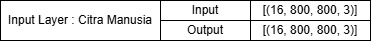
\includegraphics[scale=0.6]{gambar/inputlayerbab4.jpg}
    \caption{Input Layer Pelatihan Pertama}
    \label{fig:Input Layer Pelatihan Pertama}
\end{figure}

Pelatihan dilakukan selama 100 epoch pertama dengan ukuran batch sebesar 16 piksel, dan data diubah ukurannya menjadi 800 x 800 piksel selama preprocessing. Tujuan dari pelatihan ini adalah untuk mengevaluasi seberapa besar peningkatan performa model terlatih sebelumnya dalam mendeteksi manusia berdasarkan jumlah epoch yang dilakukan. Pada akhir 100 epoch, nilai box loss yang dihasilkan adalah 0,82978, yang menunjukkan kemampuan model untuk memprediksi bounding box dengan baik di sekitar objek. Penurunan nilai box loss selama pelatihan menunjukkan bahwa model berhasil belajar mengidentifikasi koordinat bounding box secara akurat.

\begin{figure}[H]
    \centering
    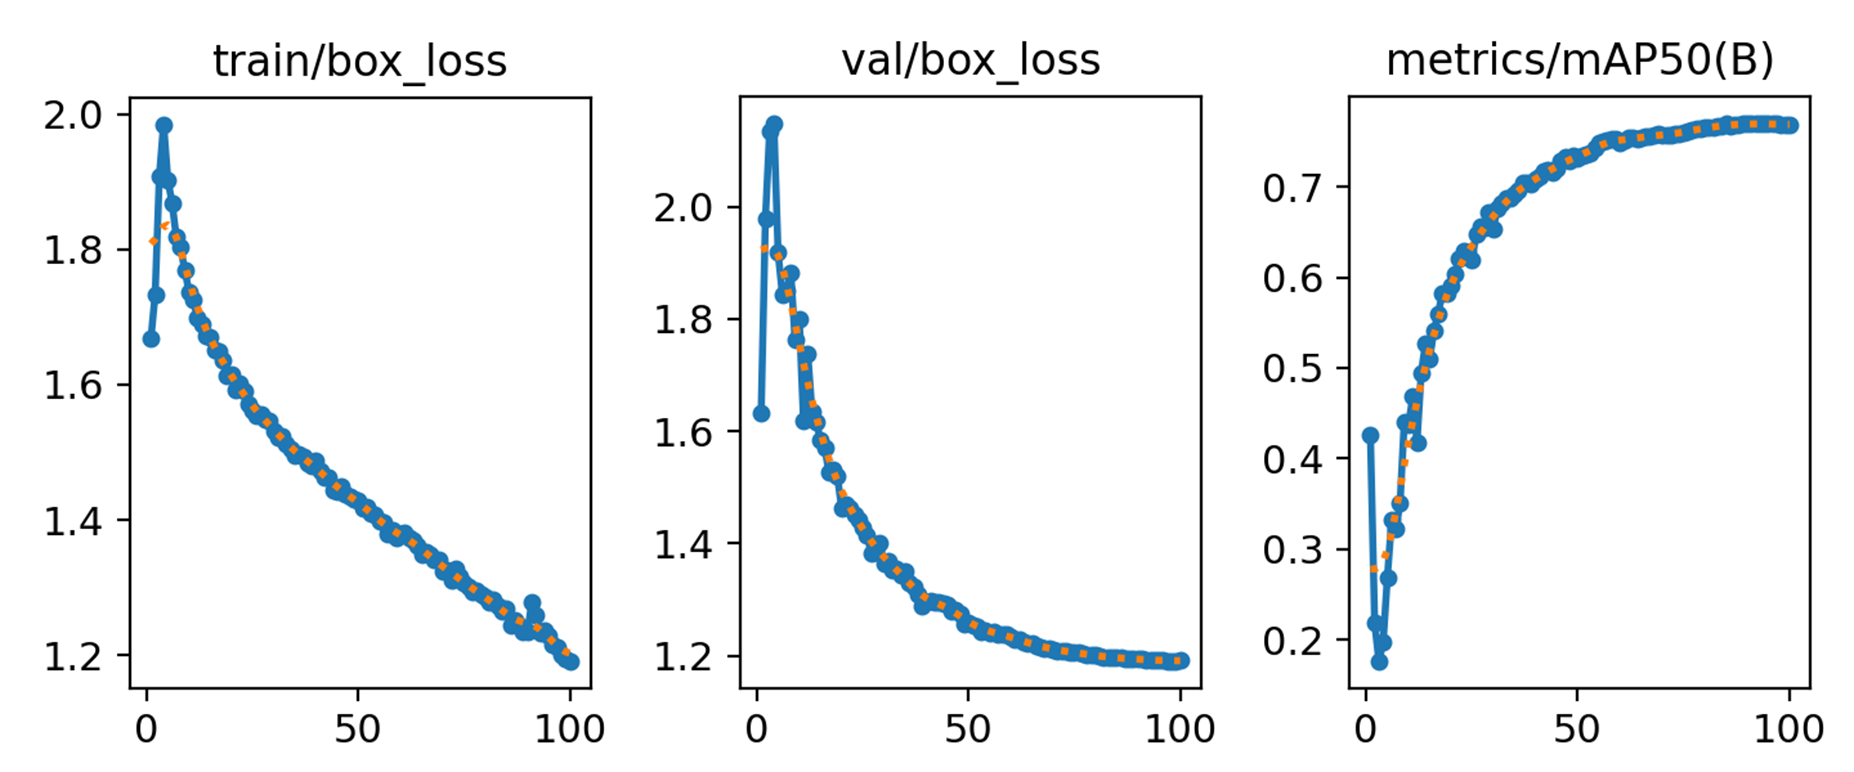
\includegraphics[scale=0.4]{gambar/loss.png}
    \caption{Loss Plot}
    \label{fig:Loss Plot}
\end{figure}

Selama validasi, nilai box loss tercatat sebesar 1,199, yang mengindikasikan kemampuan model dalam mengenali objek pada data uji. Penurunan box loss pada tahap validasi mencerminkan kemampuan model untuk mendeteksi objek secara general, tidak hanya pada data latih. Nilai mAP score divisualisasikan pada Gambar, dengan hasil skor mAP sebesar 81,85% untuk IoU minimum 0,5, yang menegaskan akurasi tinggi dalam mendeteksi objek.

Secara keseluruhan, hasil pelatihan model dirangkum pada Gambar. Nilai box loss pada pelatihan adalah 0,82978, nilai cls loss adalah 0,57615, dan dfl loss sebesar 1,1197. Metrik lainnya meliputi precision (0,84974), recall (0,72608), mAP50 (0,81855), dan mAP50-95 (0,53527). Selama validasi, nilai box loss tercatat sebesar 1,199, cls loss sebesar 0,86314, dan dfl loss sebesar 1,4956.

\begin{figure}[H]
    \centering
    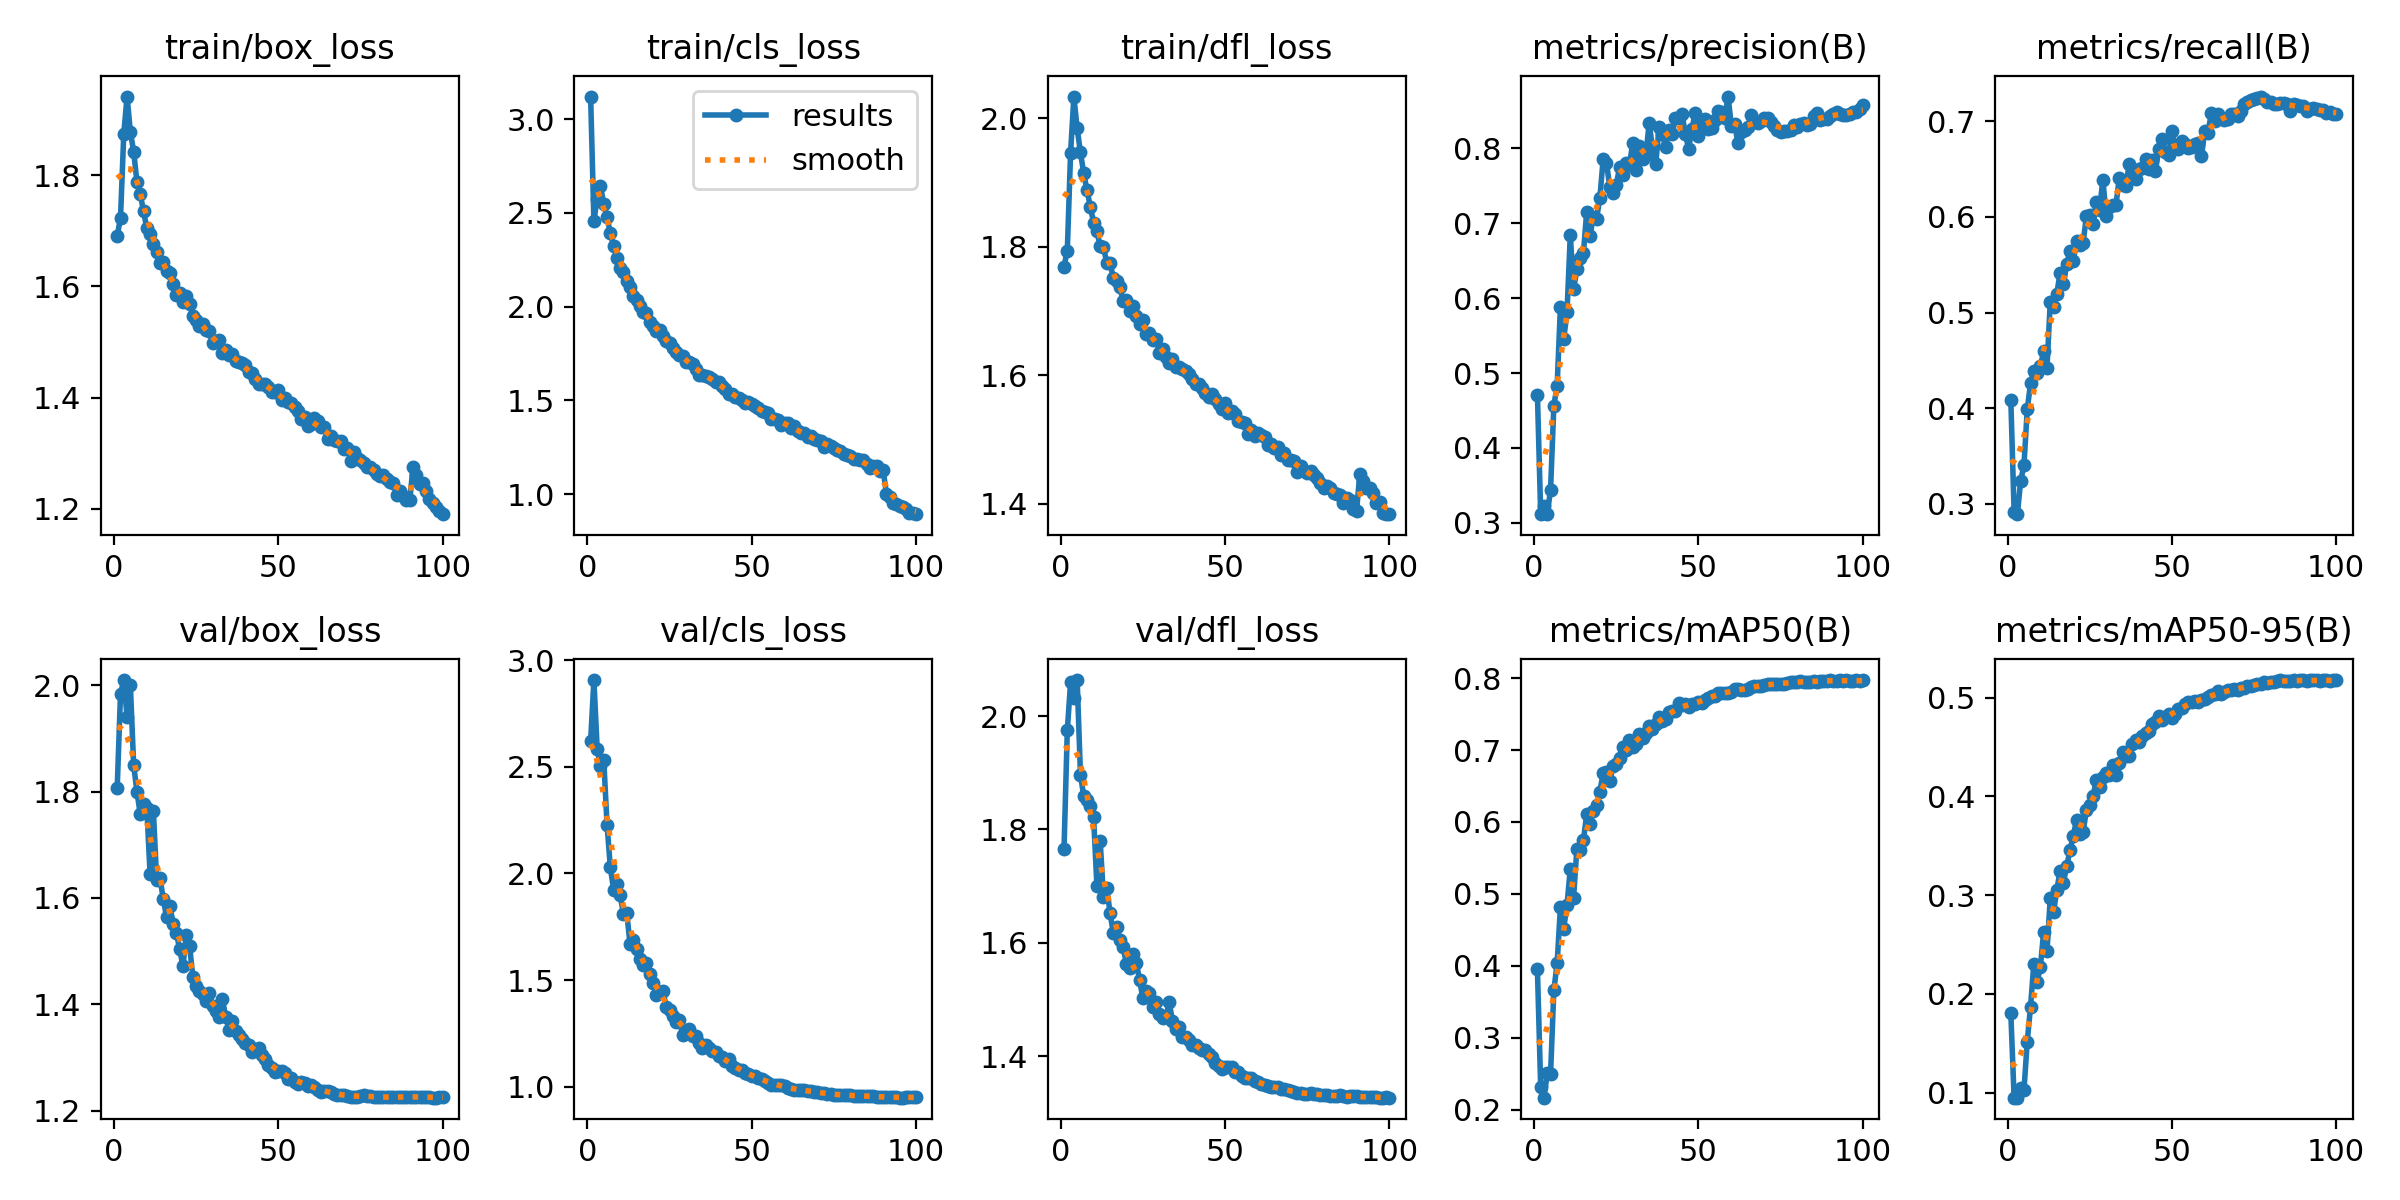
\includegraphics[scale=0.4]{gambar/results.png}
    \caption{Summary of Training Results}
    \label{fig:Summary of Training Results}
\end{figure}

Visualisasi hasil model disajikan melalui confusion matrix yang menggambarkan kinerja deteksi secara rinci. Matrix ini menunjukkan 1.806 data sebagai True Positive (manusia terdeteksi dengan benar), 483 data sebagai False Positive (objek salah terdeteksi sebagai manusia), dan 475 data sebagai False Negative (manusia yang tidak terdeteksi).

\begin{figure}[H]
    \centering
    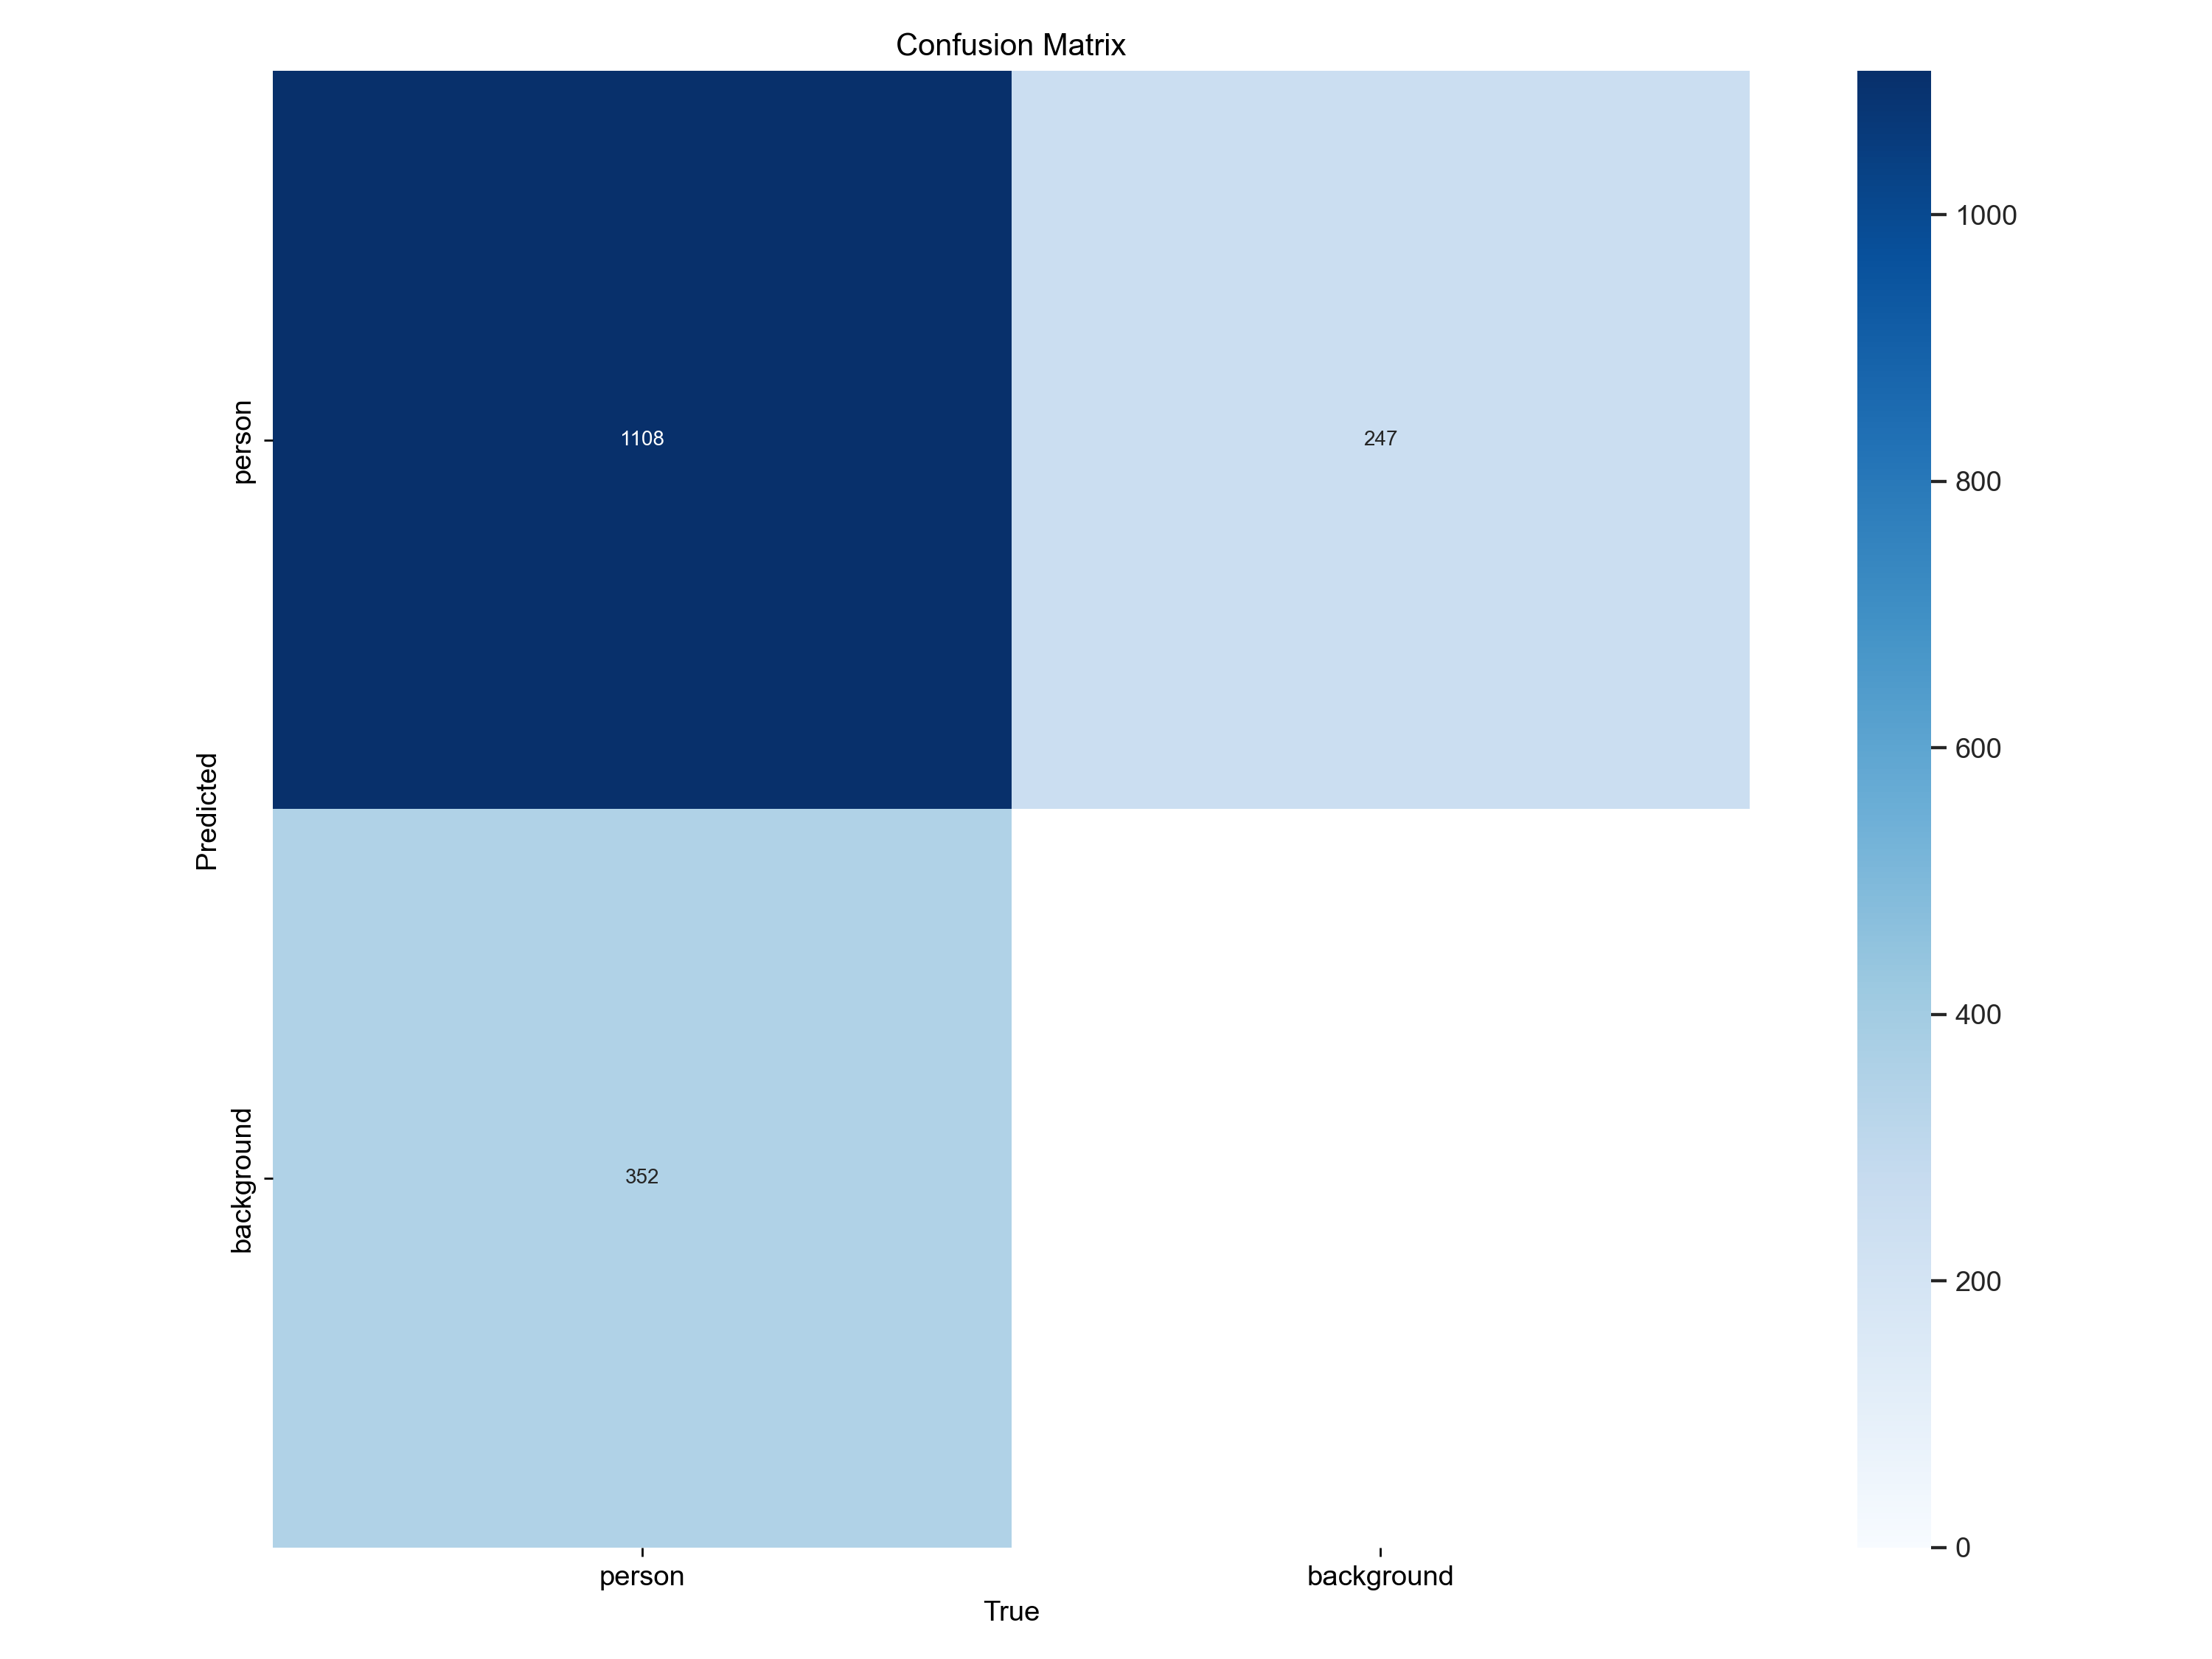
\includegraphics[scale=0.4]{gambar/confusion_matrix.png}
    \caption{Confusion Matrix}
    \label{fig:Confusion Matrix}
\end{figure}

Kurva F1-Confidence yang dihasilkan selama pelatihan menunjukkan hubungan antara confidence score dan F1-score. Model mencapai nilai F1-score tertinggi sebesar 0,78 pada confidence score 0,450, mengindikasikan keseimbangan optimal antara precision dan recall. Namun, kurva menunjukkan penurunan signifikan setelah confidence score mencapai sekitar 0,8, yang menandakan bahwa pada tingkat confidence yang sangat tinggi, model cenderung mengabaikan banyak true positives, sehingga menurunkan F1-score keseluruhan.

\begin{figure}[H]
    \centering
    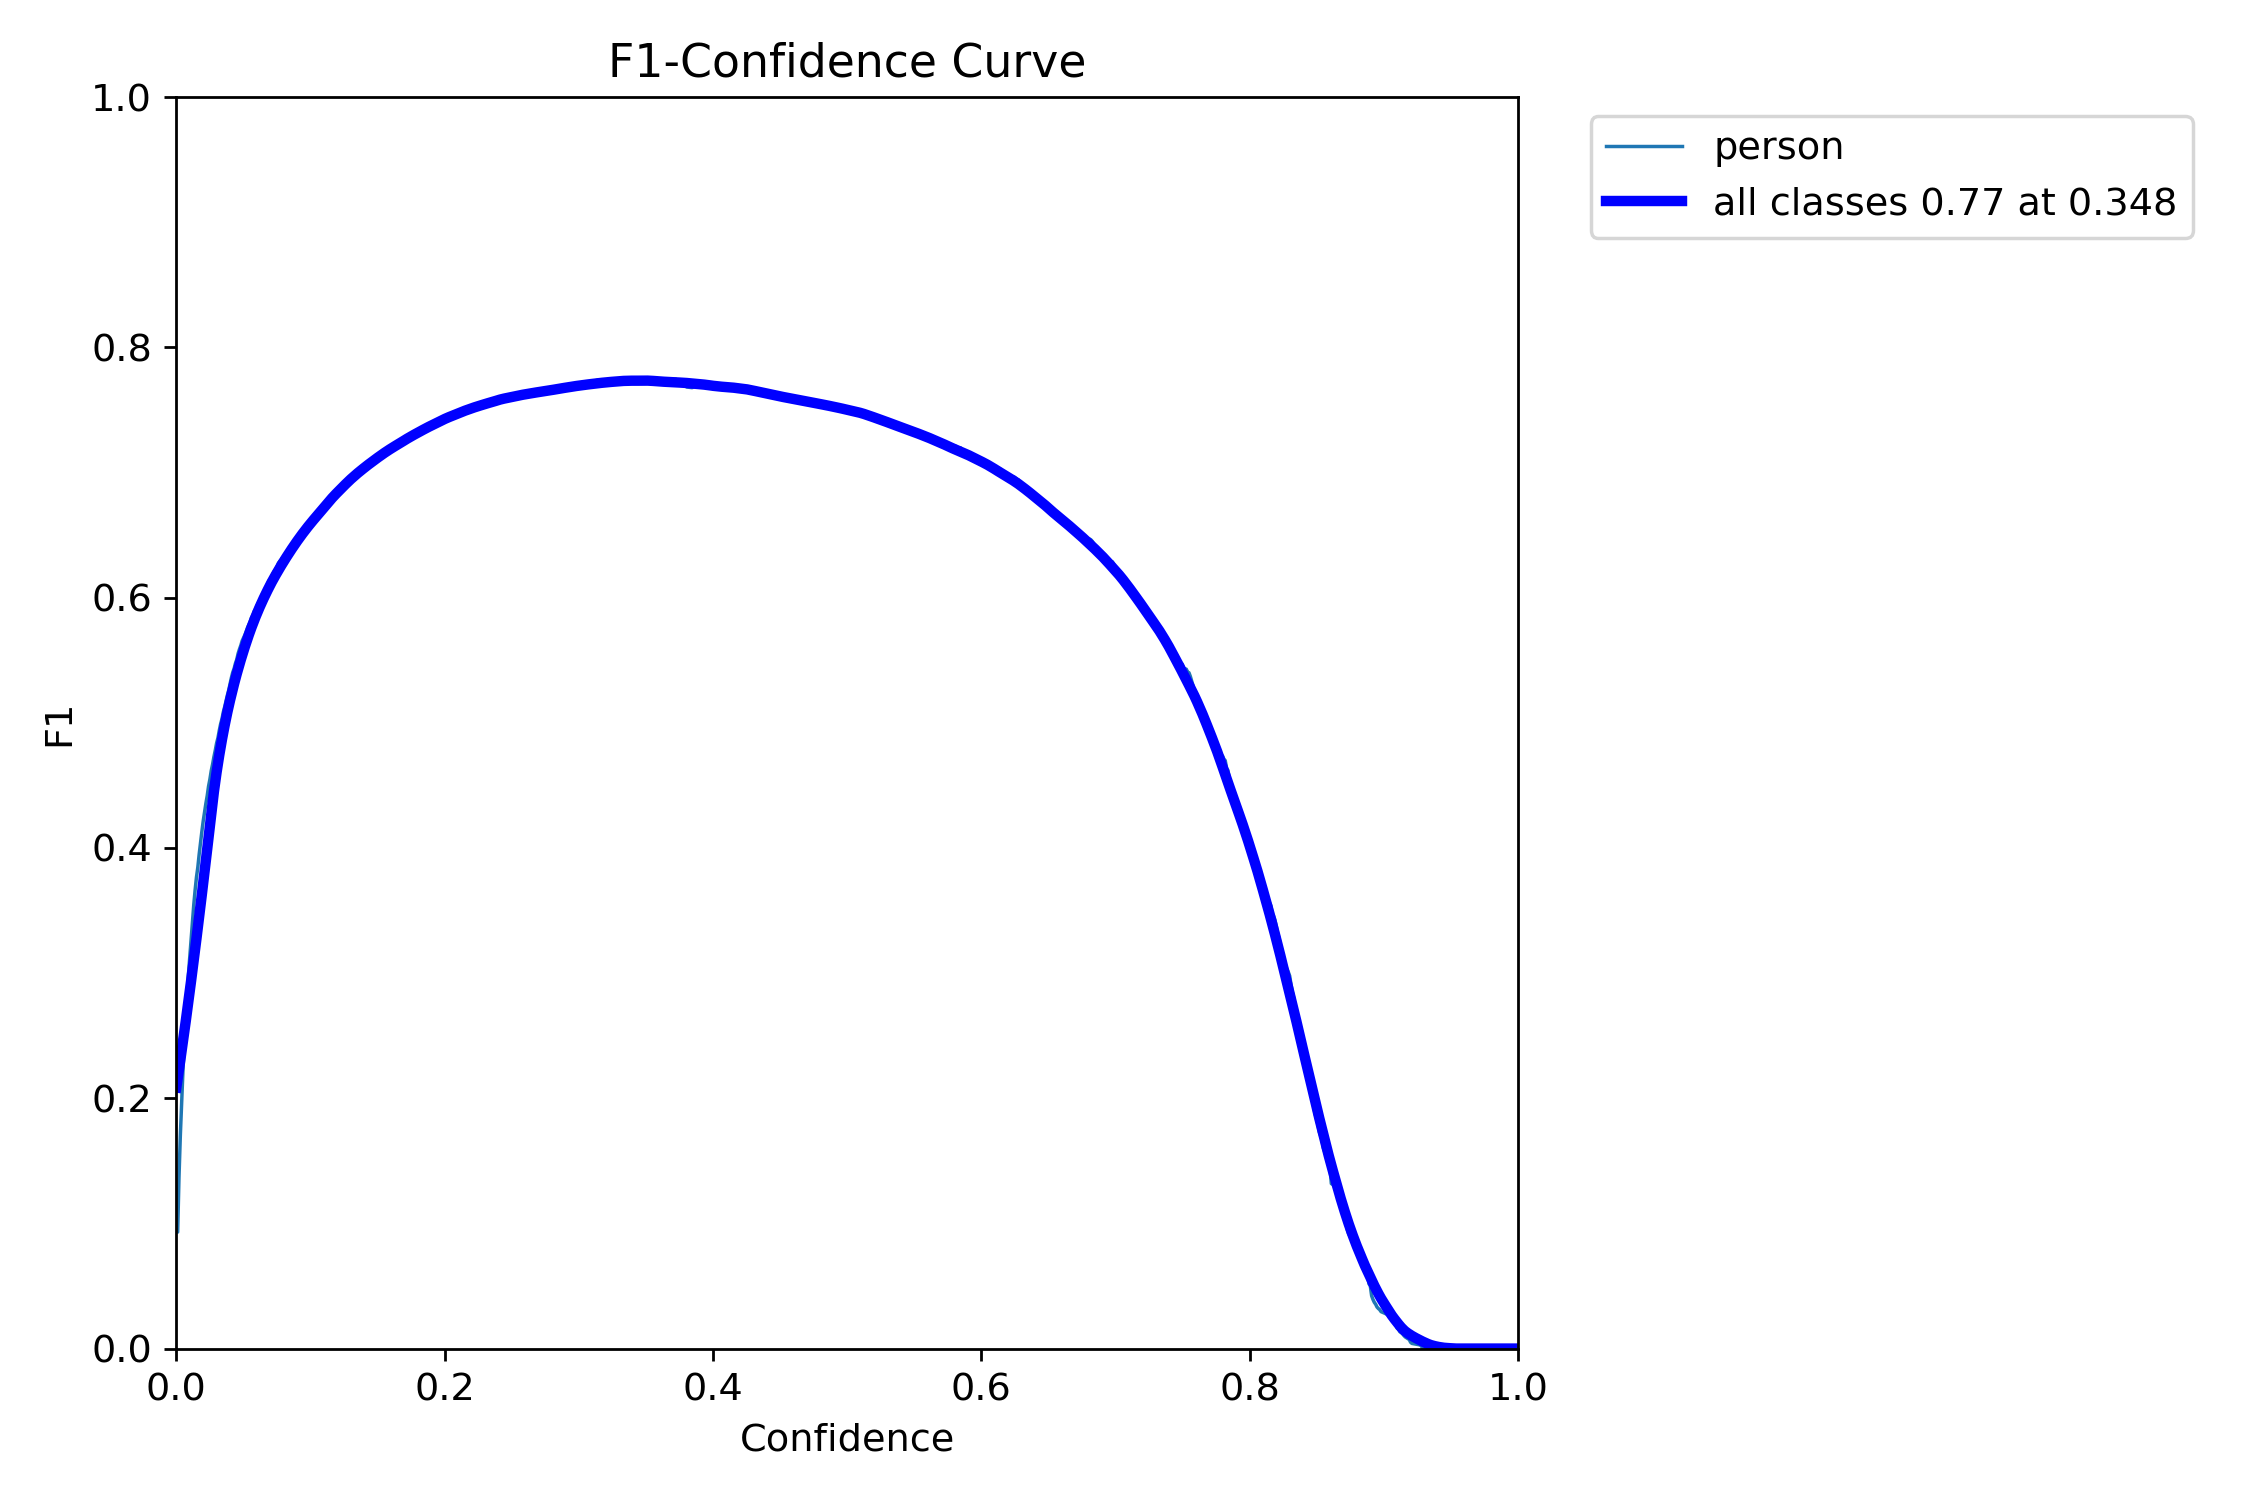
\includegraphics[scale=0.4]{gambar/F1_curve.png}
    \caption{F1-Confidence Curve}
    \label{fig:F1-Confidence Curve}
\end{figure}

Inferensi terhadap data uji juga dilakukan menggunakan model yang telah dilatih. Hasilnya menunjukkan tingkat confidence yang tinggi pada deteksi objek manusia, sebagaimana divisualisasikan dalam gambar hasil pengujian

\begin{figure}[H]
    \centering
    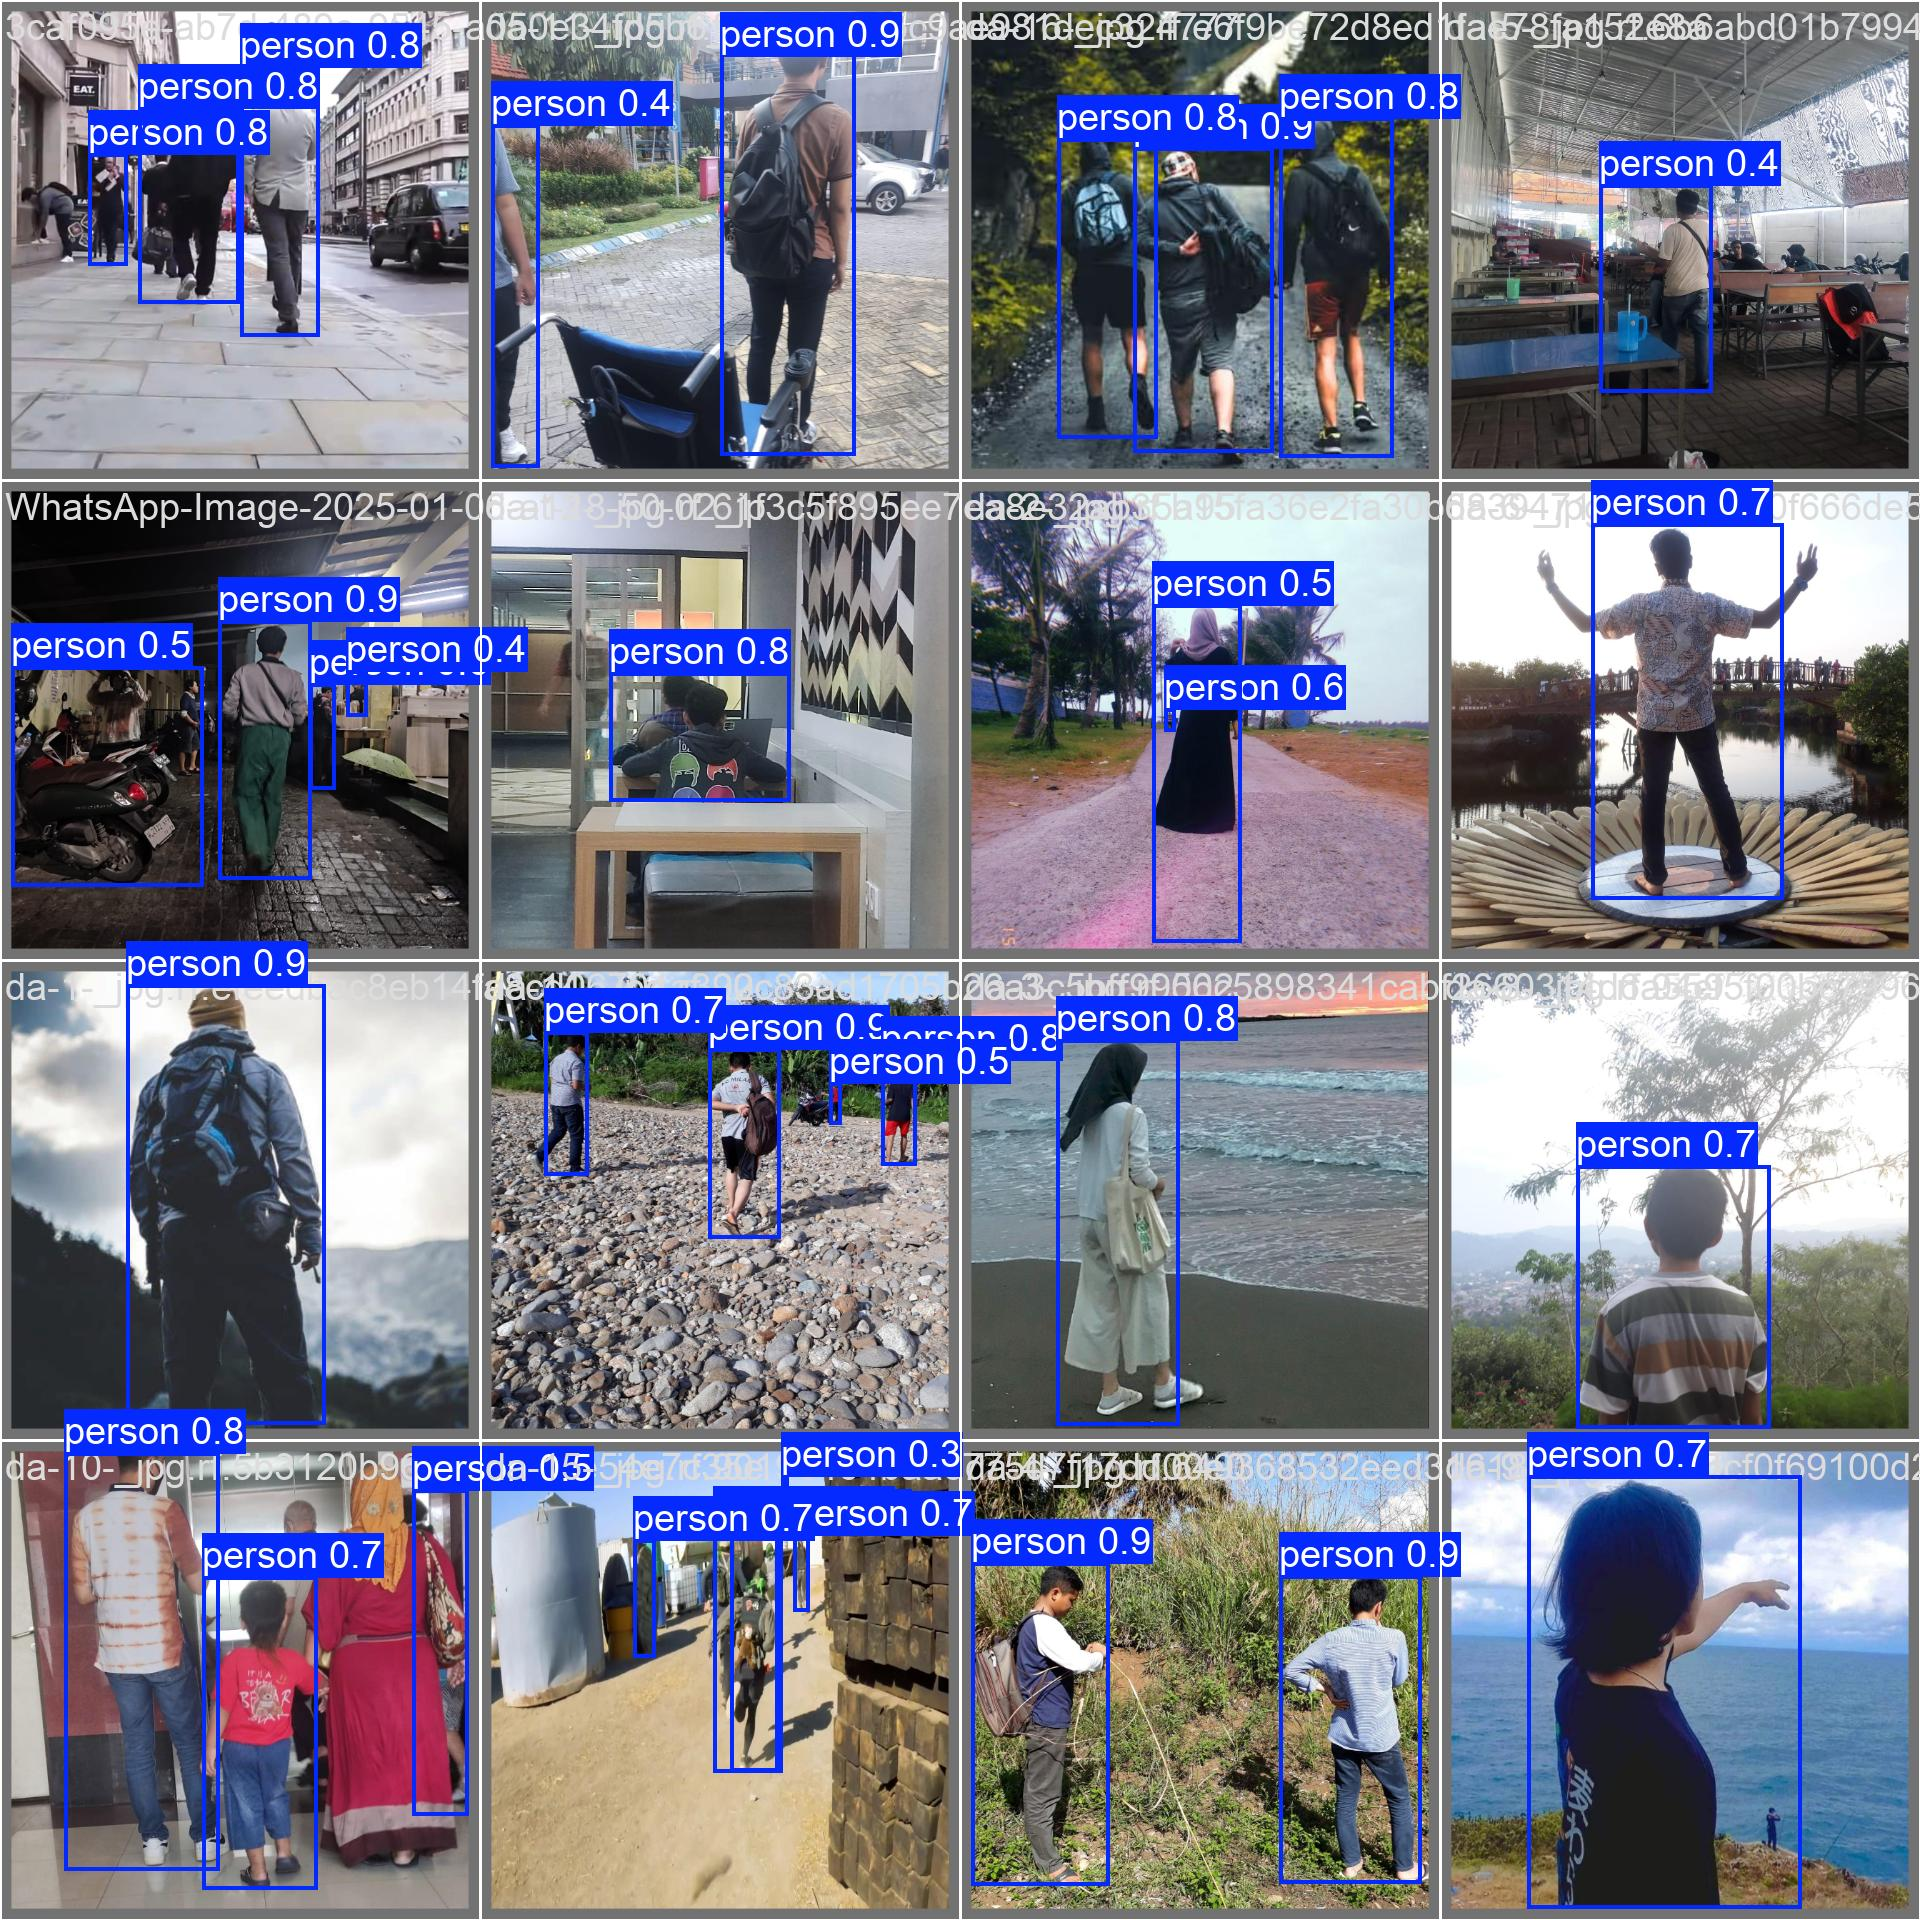
\includegraphics[scale=0.2]{gambar/pred.jpg}
    \caption{Inference Results}
    \label{fig:Inference Results}
\end{figure}

\section{Pengujian Berdasarkan FPS}
\label{sec:pengujianberdasarkanfps}
Pengujian ini dilakukan dengan menggunakan laptop MSI GF63 yang memiliki spesifikasi seperti yang tertera pada Tabel \ref{tab:spesifikasilaptop}. Laptop ini digunakan sebagai unit kontrol untuk menjalankan program dan mengirimkan instruksi ke unit eksekusi.

\begin{table}[H]
    \centering
    \caption{Spesifikasi Laptop MSI GF63 untuk Unit Kontrol}
    \label{tab:spesifikasilaptop}
    \begin{tabular}{|l|l|}
        \hline
        \rowcolor[HTML]{C0C0C0}
        \textbf{Komponen} & \textbf{Spesifikasi}  \\
        \hline
        Model Laptop            & MSI GF63                                 \\ \hline
        Prosesor                & Intel Core i7-10750H, 6 core, 12 threads \\ \hline
        GPU                     & NVIDIA RTX 3050                          \\ \hline
        RAM                     & 16GB DDR4, 3200 MHz                      \\ \hline
    \end{tabular}
\end{table}

Output yang dihasilkan setiap kali sistem memproses frame diperoleh dari verbose yang mencatat detail penting, seperti resolusi frame, jumlah objek yang terdeteksi, dan waktu pemrosesan dalam milidetik untuk setiap frame. Dalam pengujian ini, hanya 30 data pertama yang diambil dari hasil verbose tersebut untuk dianalisis lebih lanjut guna mengevaluasi konsistensi dan performa sistem dalam mendeteksi objek secara real-time.

\begin{lstlisting}[language=c]
0: 480x640 1 person, 16.0ms
0: 480x640 1 person, 23.5ms
0: 480x640 1 person, 36.0ms
0: 480x640 1 person, 18.0ms
0: 480x640 1 person, 17.5ms
\end{lstlisting}

Dari grafik \ref{fig:fps_trend}, terlihat bahwa sistem mampu mencapai FPS tertinggi sebesar 62,5 dan FPS terendah sebesar 23,81. Fluktuasi ini disebabkan oleh variasi waktu pemrosesan (dalam milidetik) untuk setiap frame, yang dipengaruhi oleh kondisi lingkungan, kompleksitas objek yang terdeteksi, dan performa perangkat keras yang digunakan.
Hasil ini menunjukkan bahwa sistem secara konsisten dapat memproses frame dengan rata-rata FPS di atas 40. Kestabilan nilai pada laptop menandakan bahwa performa sistem yang dijalankan pada laptop berjalan dengan sangat baik dan efisien.

\begin{figure}[H]
    \centering
    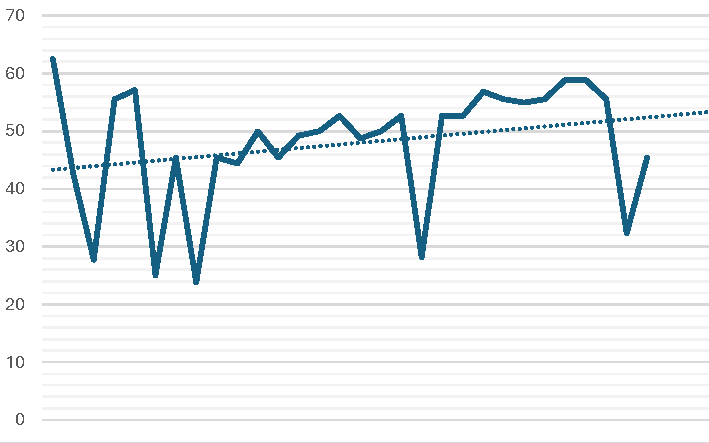
\includegraphics[width=.6\textwidth]{gambar/tex/fps.pdf}
    \caption{FPS Trend}
    \label{fig:fps_trend}
\end{figure}

\newpage
\section{Pengujian Berdasarkan Regulator Time}
\label{sec:pengujianberdasarkanregulatorsetime}

Bagian ini mengukur waktu yang dibutuhkan sistem untuk meregulasi setiap perubahan lingkungan atau perintah yang diterima.
Output yang dihasilkan setiap kali pengiriman data berisi Arah dan time stamp pada Ardruino IDE dan Visual Studio code. Berikut merupakan contoh data mentah untuk kedua hasil output: 
\begin{lstlisting}[language=c]
22:18:32.273 -> Stop
22:18:32.948 -> Arah : E
22:18:33.131 -> Kanan
22:18:33.759 -> Arah : C
22:18:33.936 -> Stop
22:18:34.748 -> Arah : B
22:18:35.121 -> Maju
22:18:35.439 -> Arah : C
22:18:35.815 -> Stop
22:18:36.410 -> Arah : E
22:18:36.616 -> Kanan
\end{lstlisting}


Output yang didapatkan pada ardruino berisikan Timestamp. Timestamp yang dihasilkan yaitu \emph{Timestamp Receive ESP} dan \emph{Timestamp Receive Motor}. Selain pada ardruino pada vscode juga didapatkan nilai time stamp \emph{sent}, contoh outputnya dapat dilihat sebagai berikut.

\begin{lstlisting}[language=python]
BELOK KANAN,0.8,2024-05-08 22:18:14.263
MAJU,0.4,2024-05-08 22:18:18.762
BELOK KANAN,0.0,2024-05-08 22:18:28.614
MAJU,0.0,2024-05-08 22:18:30.940
BELOK KANAN,1.2,2024-05-08 22:18:32.899
MAJU,0.8,2024-05-08 22:18:34.728
BELOK KANAN,0.0,2024-05-08 22:18:36.392
\end{lstlisting}

Data yang dihasilkan selama pengujian kemudian diolah dan divisualisasikan dalam bentuk plot untuk mempermudah analisis. Plot ini menunjukkan distribusi waktu yang dibutuhkan oleh sistem untuk merespons setiap perintah yang diterima.

\begin{figure}[H]
    \centering
    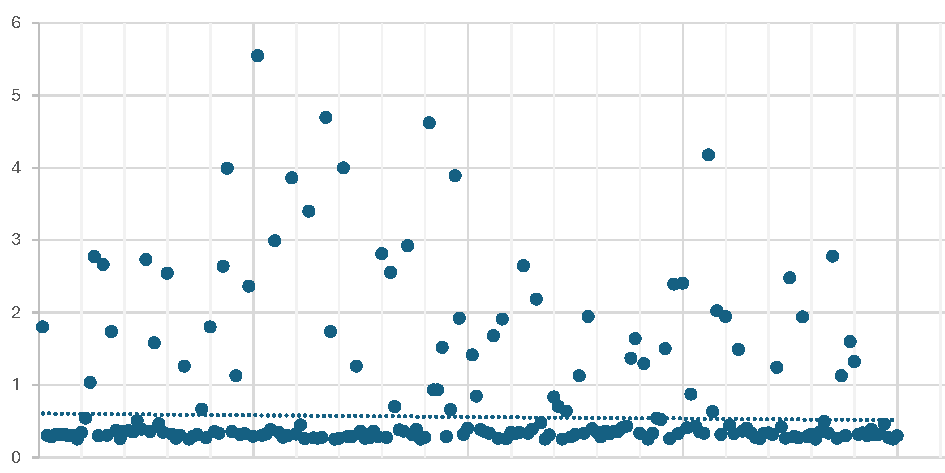
\includegraphics[width=.6\textwidth]{gambar/tex/plot.pdf}
    \caption{Regulator Time Plot}
    \label{fig:regulator_time_plot}
\end{figure}

Plot menunjukkan bahwa sekitar 66,17\% dari seluruh pengujian mampu merespons dengan cepat, berada dalam waktu yang relatif singkat.
Persentase ini menunjukkan performa sistem yang cukup baik dalam hal kecepatan respons terhadap perubahan lingkungan atau perintah. Namun, sisa 34\% data yang berada di atas 0,5 detik menunjukkan adanya variasi atau potensi keterlambatan.
% Distribusi ini dapat menjadi indikator yang baik untuk mengevaluasi stabilitas dan konsistensi sistem dalam pengujian lebih lanjut.

\newpage
\section{Pengujian Keberhasilan Tracking}
\label{sec:pengujiankeberhasiltracking}

Bagian ini mengevaluasi keberhasilan sistem dalam melakukan tracking terhadap objek target. Pengujian ini dilakukan dengan 15 kali percobaan untuk mengukur keandalan sistem dalam menjaga deteksi terhadap objek target secara konsisten. Tingkat keberhasilan diukur berdasarkan keberhasilan sistem dalam mengunci deteksi objek target (Locked Detection) atau kehilangan fokus pada objek target (Distracted Detection).

Tabel \ref{tab:tracking_success} menunjukkan data keberhasilan tracking selama pengujian. Data ini mencakup hasil tracking pada setiap percobaan, yang divisualisasikan dalam bentuk tabel dengan kode warna. Warna hijau menunjukkan bahwa sistem berhasil mengunci deteksi objek, sedangkan warna merah menunjukkan bahwa sistem gagal mengunci deteksi objek. Data ini memberikan gambaran kinerja sistem dalam mengikuti objek target, termasuk kecepatan respons, akurasi deteksi, dan ketepatan instruksi yang dikirimkan.

\begin{table}[H]
    \centering
    \caption{Data Tracking Success}
    \label{tab:tracking_success}
    \begin{tabular}{|c|c|}
        \hline 
        \cellcolor[HTML]{C0C0C0}Trial & \cellcolor[HTML]{C0C0C0}Result \\ \hline
        1 & \cellcolor[HTML]{7cFF7c}Locked Detection \\ \hline
        2 & \cellcolor[HTML]{7cFF7c}Locked Detection \\ \hline
        3 & \cellcolor[HTML]{FF7c7c}Distracted Detection \\ \hline
        4 & \cellcolor[HTML]{FF7c7c}Distracted Detection \\ \hline
        5 & \cellcolor[HTML]{FF7c7c}Distracted Detection \\ \hline
        6 & \cellcolor[HTML]{FF7c7c}Distracted Detection \\ \hline
        7 & \cellcolor[HTML]{7cFF7c}Locked Detection \\ \hline
        8 & \cellcolor[HTML]{7cFF7c}Locked Detection \\ \hline
        9 & \cellcolor[HTML]{FF7c7c}Distracted Detection \\ \hline 
        10 & \cellcolor[HTML]{FF7c7c}Distracted Detection \\ \hline
        11 & \cellcolor[HTML]{FF7c7c}Distracted Detection \\ \hline
        12 & \cellcolor[HTML]{FF7c7c}Distracted Detection \\ \hline
        13 & \cellcolor[HTML]{FF7c7c}Distracted Detection \\ \hline
        14 & \cellcolor[HTML]{FF7c7c}Distracted Detection \\ \hline
        15 & \cellcolor[HTML]{FF7c7c}Distracted Detection \\ \hline
    \end{tabular}
\end{table}

Kemampuan BotSORT pada YOLO dalam melakukan tracking objek manusia terlihat dari 15 kali percobaan. Sistem berhasil mengunci deteksi objek sebanyak 4 kali, sedangkan 11 kali gagal mengunci deteksi objek secara akumulasi. Hasil ini menunjukkan bahwa sistem mampu melakukan tracking objek dengan tingkat keberhasilan sebesar 26,67\%. Namun, terdapat 73,33\% kegagalan dalam mengunci deteksi objek, yang menunjukkan adanya kekurangan dalam sistem.

Hasil ini menunjukkan bahwa sistem masih memiliki keterbatasan dalam menjaga stabilitas pelacakan terhadap objek target secara konsisten. Ketidakkonsistenan dalam pelacakan objek sering kali menyebabkan sistem kehilangan fokus pada target dan menghasilkan nomor ID baru untuk setiap deteksi ulang. Namun, meskipun terjadi kegagalan pelacakan, penggunaan ID terkecil memungkinkan identifikasi objek tetap dilakukan dengan tingkat akurasi yang memadai. Pendekatan ini membantu proses pengujian tetap berjalan dengan acuan identitas objek yang konsisten meskipun terdapat keterbatasan dalam menjaga kesinambungan pelacakan.

\begin{figure}[H]
    \centering
  
    % Ubah dengan nama file gambar dan ukuran yang akan digunakan
    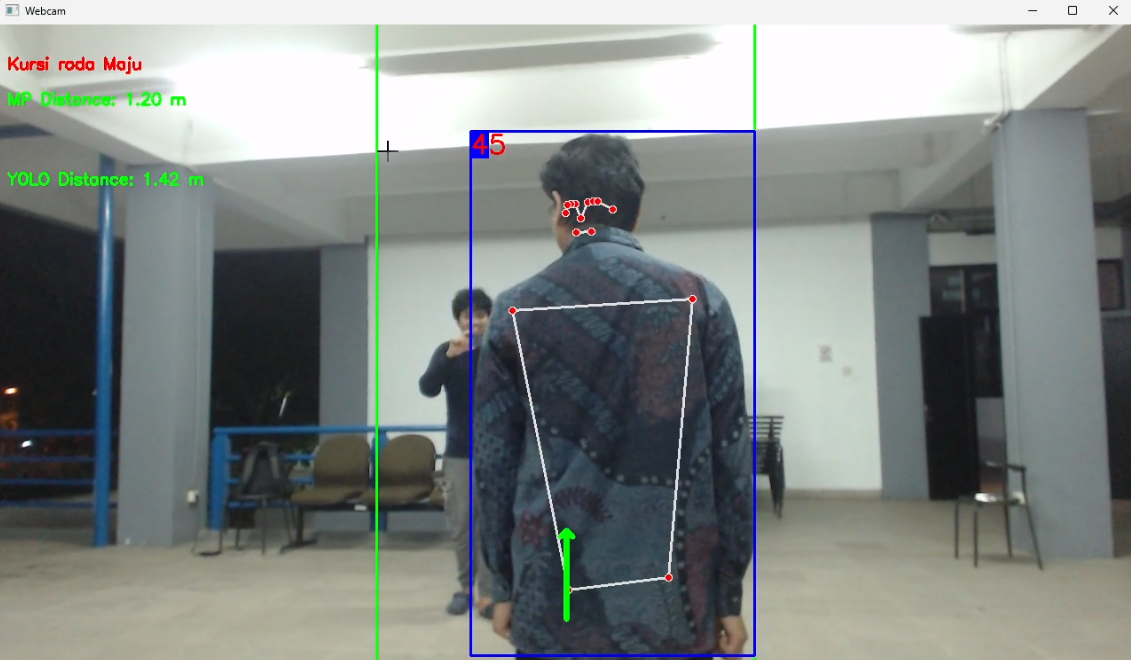
\includegraphics[scale=0.4]{gambar/Track.png}

    \caption{Tracking Numeral}
    \label{fig:tracking_numeral}
\end{figure}

Gambar \ref{fig:tracking_numeral} menunjukkan peningkatan nomor track yang terus bertambah. Hal ini disebabkan oleh performa yang kurang optimal dari fungsi \texttt{model.track()} pada YOLO. Ketidakmampuan model untuk secara konsisten melacak objek menyebabkan nomor track baru dibuat setiap kali objek gagal terdeteksi, sehingga menghasilkan peningkatan jumlah track yang tidak diinginkan. 
Akan tetapi penguncian ini masih bisa digunakan walau tidak seperti satu id tiap object dan masih bisa digunakan dengan id terkecil sebagai penguncian. Hal ini menunjukkan bahwa meskipun sistem tidak selalu memberikan ID yang konsisten untuk setiap objek, ID terkecil yang diberikan dapat digunakan sebagai referensi untuk penguncian objek. Dengan demikian, sistem masih dapat melacak objek dengan tingkat keberhasilan tertentu meskipun terdapat beberapa kekurangan dalam konsistensi ID.


\section{Pengujian Tingkat Pencahayaan}
\label{sec:pengujiantingkatpencahayaan}

Pengujian dilakukan untuk mengukur kemampuan sistem dalam mendeteksi objek pada berbagai tingkat pencahayaan. Fokus pengujian ini adalah memastikan bahwa sistem dapat berfungsi dengan baik dalam kondisi pencahayaan yang berbeda.

\begin{table}[H]
    \centering
    \caption{Lighting Level Evaluation}
    \label{tab:lighting_level_evaluation}
    \begin{tabular}{|c|c|c|c|c|c|}
        \hline 
        \rowcolor[HTML]{C0C0C0} 
        \multicolumn{1}{|c|}{\cellcolor[HTML]{C0C0C0}}& \multicolumn{3}{c|}{\cellcolor[HTML]{C0C0C0}\textbf{Lux}} & \multicolumn{2}{c|}{\cellcolor[HTML]{C0C0C0}\textbf{Conf.}}  \\ \cline{2-6} 
        \rowcolor[HTML]{C0C0C0} 
        \multicolumn{1}{|c|}{\multirow{-2}{*}{\cellcolor[HTML]{C0C0C0}\textbf{Time of Day}}} & \multicolumn{1}{c|}{\cellcolor[HTML]{C0C0C0}\textbf{Min}} & \multicolumn{1}{c|}{\cellcolor[HTML]{C0C0C0}\textbf{Avg}} & \multicolumn{1}{c|}{\cellcolor[HTML]{C0C0C0}\textbf{Max}} & \multicolumn{1}{c|}{\cellcolor[HTML]{C0C0C0}\textbf{YOLO}} & \multicolumn{1}{c|}{\cellcolor[HTML]{C0C0C0}\textbf{MP}} \\ \hline
        \cellcolor[HTML]{C0C0C0} \textbf{Morning} & 100 & 300 & 500 & 0.73 & 0.71 \\ \hline
        \cellcolor[HTML]{C0C0C0} \textbf{Afternoon} & 2622 & 3753 & 5574 & 0.82 & 0.76 \\ \hline
        \cellcolor[HTML]{C0C0C0} \textbf{Evening} & 50 & 200 & 400 & 0.75 & 0.70 \\ \hline
        \cellcolor[HTML]{C0C0C0} \textbf{Night} & 26 & 215 & 538 & 0.60 & 0.56 \\ \hline
    \end{tabular}
\end{table}

Tabel \ref{tab:lighting_level_evaluation} menunjukkan data tingkat pencahayaan yang diukur pada berbagai waktu sepanjang hari. Data ini mencakup tingkat pencahayaan minimum, rata-rata, dan maksimum yang diukur dalam lux, serta tingkat kepercayaan deteksi yang dihasilkan oleh YOLOv11 dan MediaPipe Pose. Data ini memberikan gambaran kinerja sistem dalam berbagai kondisi pencahayaan, termasuk akurasi deteksi, kecepatan respons, dan ketepatan instruksi yang dikirimkan.

\newpage
\section{Pengujian Kesesuaian Jarak Deteksi}
\label{sec:pengujiankesesuaianjarakdeteksi}

Pengujian dilakukan untuk mengukur kemampuan sistem dalam mendeteksi objek pada berbagai jarak dan menganalisis performa sistem pada jarak-jarak tersebut. Fokus pengujian ini adalah memastikan bahwa ketika objek berada pada jarak yang sangat dekat (\textless 1m), sistem mengirimkan kode instruksi untuk berhenti (diam) guna mencegah tabrakan.

\begin{table}[H]
    \centering
    \caption{Data Jarak (\textless 1m) untuk Diam}
    \label{tab:jarak_diam}
    \begin{tabular}{|c|c|c|c|c|c|c|c|c|}
    \hline
    Waktu & Reg (s) & YOLO (m) & MP (m) & x (px) & Deteksi & Terkirim & Keterangan \\ \hline
    12:55:12 & 0.8402 & 2.0631 & 0.9852 & 833 & b'C\textbackslash n' & b'C\textbackslash n' & Stop \\ \hline
    12:55:15 & 0.2585 & 1.1003 & 0.8942 & 242 & b'C\textbackslash n' & b'C\textbackslash n' & Stop \\ \hline
    12:55:24 & 2.1821 & 1.1773 & 0.9652 & 511 & b'C\textbackslash n' & b'C\textbackslash n' & Stop \\ \hline
    12:58:13 & 1.4998 & 1.4123 & 0.9574 & 531 & b'C\textbackslash n' & b'C\textbackslash n' & Stop \\ \hline
    12:58:14 & 0.2538 & 1.4538 & 0.9899 & 555 & b'C\textbackslash n' & b'C\textbackslash n' & Stop \\ \hline
    12:58:19 & 2.4033 & 1.1691 & 0.9213 & 852 & b'C\textbackslash n' & b'C\textbackslash n' & Stop \\ \hline
    12:58:19 & 0.4079 & 1.1839 & 0.9118 & 854 & b'C\textbackslash n' & b'C\textbackslash n' & Stop \\ \hline
    12:58:20 & 0.8708 & 1.0960 & 0.9548 & 528 & b'C\textbackslash n' & b'C\textbackslash n' & Stop \\ \hline
    12:58:21 & 0.4262 & 1.1003 & 0.9189 & 547 & b'C\textbackslash n' & b'C\textbackslash n' & Stop \\ \hline
    12:58:21 & 0.3497 & 1.1032 & 0.8985 & 554 & b'C\textbackslash n' & b'C\textbackslash n' & Stop \\ \hline
    12:58:21 & 0.3314 & 1.1032 & 0.8785 & 518 & b'C\textbackslash n' & b'C\textbackslash n' & Stop \\ \hline
    13:00:57 & 1.4848 & 1.1594 & 0.9943 & 208 & b'C\textbackslash n' & b'C\textbackslash n' & Stop \\ \hline
    13:01:15 & 1.5987 & 1.3643 & 0.9899 & 849 & b'C\textbackslash n' & b'C\textbackslash n' & Stop \\ \hline
    13:01:19 & 0.2719 & 1.0989 & 0.7700 & 856 & b'C\textbackslash n' & b'C\textbackslash n' & Stop \\ \hline
    13:01:19 & 0.2509 & 1.1452 & 0.5782 & 856 & b'C\textbackslash n' & b'C\textbackslash n' & Stop \\ \hline
    17:41:34 & 0.3036 & 1.4339 & 0.9447 & 647 & b'C\textbackslash n' & b'C\textbackslash n' & Stop \\ \hline
    17:41:35 & 0.3326 & 1.4291 & 0.8357 & 642 & b'C\textbackslash n' & b'C\textbackslash n' & Stop \\ \hline
    17:41:36 & 0.3588 & 1.4389 & 0.8222 & 672 & b'C\textbackslash n' & b'C\textbackslash n' & Stop \\ \hline
    17:41:45 & 0.3092 & 1.3913 & 0.7249 & 640 & b'C\textbackslash n' & b'C\textbackslash n' & Stop \\ \hline
    17:42:04 & 15.5192 & 1.4563 & 0.5955 & 213 & b'C\textbackslash n' & b'C\textbackslash n' & Stop \\ \hline
    \end{tabular}
    \end{table}

Tabel \ref{tab:jarak_diam} menunjukkan data jarak yang diukur ketika objek berada pada jarak kurang dari 1 meter. Data ini mencakup waktu deteksi, jarak deteksi dari YOLOv11 dan MediaPipe Pose, posisi objek dalam frame, hasil deteksi, instruksi yang dikirimkan, dan keterangan mengenai status objek. Data ini memberikan gambaran kinerja sistem dalam mengikuti objek yang berada pada jarak dekat, termasuk kecepatan respons, akurasi deteksi, dan ketepatan instruksi yang dikirimkan.

Pengujian jarak juga telah diverifikasi secara fisik dengan pengukuran dan perbandingan yang cermat sebelum menyajikan data. Hal ini memastikan akurasi dan keandalan pengukuran jarak yang digunakan dalam evaluasi. Proses verifikasi melibatkan penggunaan alat ukur yang terkalibrasi dan uji coba berulang untuk meminimalkan kesalahan.

\newpage
\section{Performa Pergerakan Mengikuti Objek}
\label{sec:performaakurasiobjek}

Analisis dilakukan untuk mengukur seberapa akurat sistem dapat mengikuti objek target, termasuk mempertahankan jarak yang tepat dan tidak kehilangan objek dalam berbagai kondisi.

\subsection{Percobaan Dalam Frame}
\label{subsec:percobaandalamframe}

Bagian ini membahas kemampuan sistem dalam mengikuti objek yang berada di dalam frame kamera dengan fokus utama pada evaluasi kinerja regulator. Tujuannya adalah memastikan bahwa sistem dapat merespons hasil deteksi dengan akurat dan konsisten, sesuai dengan kondisi objek yang terdeteksi di dalam frame kamera. Analisis dilakukan menggunakan 100 data sampel untuk memberikan gambaran kinerja sistem secara menyeluruh.

\begin{longtable}{|c|c|c|c|c|c|c|c|}
    \caption{Data Status Frame (Dalam Frame)} \label{tab:status_dalam_frame} \\
    \hline
    Waktu & Reg (s) & YOLO (m) & MP (m) & x (px) & Deteksi & Terkirim & Keterangan \\ \hline
    \endhead
    \hline \multicolumn{8}{|r|}{Lanjutan ke halaman berikutnya} \\ \hline
    \endfoot
    \endlastfoot
    12:48:09 & 0.2960 & 2.4469 & 2.6214 & 765 & b'E\textbackslash n' & b'C\textbackslash n' & Turn Right \\ \hline
12:48:09 & 0.2991 & 5.6875 & 4.1146 & 484 & b'B\textbackslash n' & b'E\textbackslash n' & Forward \\ \hline
12:48:10 & 0.2516 & 2.2093 & 2.6063 & 595 & b'B\textbackslash n' & b'C\textbackslash n' & Forward \\ \hline
12:48:14 & 2.7739 & 1.4513 & 1.7409 & 128 & b'A\textbackslash n' & b'A\textbackslash n' & Turn Left \\ \hline
12:48:17 & 2.6621 & 1.7109 & 1.1479 & 447 & b'B\textbackslash n' & b'C\textbackslash n' & Forward \\ \hline
12:50:45 & 0.5046 & 2.5900 & 1.4523 & 391 & b'B\textbackslash n' & b'B\textbackslash n' & Forward \\ \hline
12:50:48 & 2.7333 & 1.1421 & 1.9733 & 164 & b'A\textbackslash n' & b'C\textbackslash n' & Turn Left \\ \hline
12:50:51 & 0.4610 & 1.4219 & 1.0142 & 830 & b'E\textbackslash n' & b'E\textbackslash n' & Turn Right \\ \hline
12:50:54 & 2.5388 & 1.4768 & 1.1208 & 501 & b'B\textbackslash n' & b'C\textbackslash n' & Forward \\ \hline
12:50:57 & 0.2675 & 2.0939 & 1.4524 & 825 & b'E\textbackslash n' & b'E\textbackslash n' & Turn Right \\ \hline
12:51:00 & 0.3556 & 1.7144 & 1.5984 & 492 & b'B\textbackslash n' & b'C\textbackslash n' & Forward \\ \hline
12:51:00 & 0.3290 & 1.4978 & 1.4964 & 466 & b'B\textbackslash n' & b'B\textbackslash n' & Forward \\ \hline
12:51:07 & 3.9922 & 1.7796 & 1.3830 & 896 & b'E\textbackslash n' & b'C\textbackslash n' & Turn Right \\ \hline
12:51:08 & 0.3129 & 1.6801 & 1.7017 & 525 & b'B\textbackslash n' & b'C\textbackslash n' & Forward \\ \hline
12:51:09 & 0.3226 & 1.6408 & 1.7256 & 463 & b'B\textbackslash n' & b'B\textbackslash n' & Forward \\ \hline
12:51:11 & 2.3641 & 1.5332 & 1.1242 & 850 & b'E\textbackslash n' & b'C\textbackslash n' & Turn Right \\ \hline
12:51:17 & 5.5467 & 2.2628 & 1.6525 & 563 & b'B\textbackslash n' & b'C\textbackslash n' & Forward \\ \hline
12:51:17 & 0.3035 & 1.9853 & 1.6709 & 408 & b'B\textbackslash n' & b'B\textbackslash n' & Forward \\ \hline
12:51:18 & 0.3176 & 1.6668 & 1.5184 & 189 & b'A\textbackslash n' & b'C\textbackslash n' & Turn Left \\ \hline
12:51:18 & 0.3818 & 1.5277 & 1.4295 & 202 & b'A\textbackslash n' & b'A\textbackslash n' & Turn Left \\ \hline
12:51:21 & 2.9916 & 2.0186 & 1.6728 & 440 & b'B\textbackslash n' & b'C\textbackslash n' & Forward \\ \hline
12:51:21 & 0.3446 & 2.4830 & 1.6701 & 601 & b'B\textbackslash n' & b'B\textbackslash n' & Forward \\ \hline
12:51:22 & 0.2721 & 2.6141 & 1.7926 & 769 & b'E\textbackslash n' & b'C\textbackslash n' & Turn Right \\ \hline
12:51:22 & 0.2947 & 2.7330 & 1.5570 & 867 & b'E\textbackslash n' & b'E\textbackslash n' & Turn Right \\ \hline
12:51:26 & 3.8579 & 2.5354 & 1.6134 & 553 & b'B\textbackslash n' & b'C\textbackslash n' & Forward \\ \hline
12:51:26 & 0.4472 & 1.9174 & 1.2873 & 212 & b'A\textbackslash n' & b'C\textbackslash n' & Turn Left \\ \hline
12:51:27 & 0.2536 & 1.6668 & 1.9112 & 142 & b'A\textbackslash n' & b'A\textbackslash n' & Turn Left \\ \hline
12:51:30 & 3.3993 & 2.4258 & 1.4468 & 551 & b'B\textbackslash n' & b'C\textbackslash n' & Forward \\ \hline
12:51:36 & 4.6957 & 1.7144 & 1.8941 & 478 & b'B\textbackslash n' & b'B\textbackslash n' & Forward \\ \hline
12:51:37 & 1.7377 & 1.5194 & 1.8537 & 182 & b'A\textbackslash n' & b'C\textbackslash n' & Turn Left \\ \hline
12:51:42 & 0.2820 & 1.4820 & 1.5157 & 424 & b'B\textbackslash n' & b'C\textbackslash n' & Forward \\ \hline
12:51:42 & 0.2867 & 1.5473 & 1.6206 & 481 & b'B\textbackslash n' & b'B\textbackslash n' & Forward \\ \hline
12:51:44 & 0.3591 & 2.1528 & 1.7878 & 245 & b'A\textbackslash n' & b'C\textbackslash n' & Turn Left \\ \hline
12:51:44 & 0.2619 & 1.6003 & 1.9633 & 426 & b'B\textbackslash n' & b'A\textbackslash n' & Forward \\ \hline
12:51:45 & 0.2692 & 1.5704 & 1.6022 & 449 & b'B\textbackslash n' & b'C\textbackslash n' & Forward \\ \hline
12:51:45 & 0.3616 & 1.8259 & 1.5129 & 249 & b'A\textbackslash n' & b'B\textbackslash n' & Turn Left \\ \hline
12:51:48 & 2.8133 & 1.7721 & 1.1400 & 766 & b'E\textbackslash n' & b'C\textbackslash n' & Turn Right \\ \hline
12:51:48 & 0.2701 & 1.9485 & 1.8638 & 792 & b'E\textbackslash n' & b'E\textbackslash n' & Turn Right \\ \hline
12:51:51 & 2.5508 & 2.2628 & 1.9379 & 569 & b'B\textbackslash n' & b'C\textbackslash n' & Forward \\ \hline
12:51:52 & 0.6972 & 1.9174 & 1.6452 & 394 & b'B\textbackslash n' & b'B\textbackslash n' & Forward \\ \hline
12:51:52 & 0.3755 & 1.5912 & 1.3909 & 185 & b'A\textbackslash n' & b'C\textbackslash n' & Turn Left \\ \hline
12:51:52 & 0.3613 & 1.4716 & 1.2101 & 174 & b'A\textbackslash n' & b'A\textbackslash n' & Turn Left \\ \hline
12:51:55 & 0.3125 & 1.9262 & 1.1721 & 564 & b'B\textbackslash n' & b'C\textbackslash n' & Forward \\ \hline
12:51:56 & 0.3797 & 1.9667 & 1.6343 & 835 & b'E\textbackslash n' & b'B\textbackslash n' & Turn Right \\ \hline
12:51:56 & 0.2506 & 1.9262 & 1.7147 & 880 & b'E\textbackslash n' & b'C\textbackslash n' & Turn Right \\ \hline
12:51:56 & 0.2716 & 1.9759 & 1.6276 & 871 & b'E\textbackslash n' & b'E\textbackslash n' & Turn Right \\ \hline
12:52:05 & 0.2830 & 1.9395 & 1.9075 & 502 & b'B\textbackslash n' & b'C\textbackslash n' & Forward \\ \hline
12:55:09 & 1.9217 & 1.5004 & 1.8914 & 861 & b'E\textbackslash n' & b'E\textbackslash n' & Turn Right \\ \hline
12:55:10 & 0.3128 & 1.4414 & 1.8698 & 858 & b'E\textbackslash n' & b'C\textbackslash n' & Turn Right \\ \hline
12:55:10 & 0.3967 & 1.7356 & 1.0821 & 856 & b'E\textbackslash n' & b'E\textbackslash n' & Turn Right \\ \hline
12:55:13 & 0.3498 & 2.0186 & 1.9290 & 520 & b'B\textbackslash n' & b'C\textbackslash n' & Forward \\ \hline
12:55:14 & 0.3321 & 1.8664 & 1.4010 & 511 & b'B\textbackslash n' & b'B\textbackslash n' & Forward \\ \hline
12:55:15 & 1.6785 & 1.1238 & 1.0672 & 170 & b'A\textbackslash n' & b'C\textbackslash n' & Turn Left \\ \hline
12:55:18 & 0.2536 & 1.2489 & 1.0783 & 483 & b'B\textbackslash n' & b'C\textbackslash n' & Forward \\ \hline
12:55:18 & 0.3224 & 1.2129 & 1.4666 & 168 & b'A\textbackslash n' & b'C\textbackslash n' & Turn Left \\ \hline
12:55:19 & 0.3399 & 1.1515 & 1.3422 & 165 & b'A\textbackslash n' & b'A\textbackslash n' & Turn Left \\ \hline
12:55:22 & 0.3309 & 1.5194 & 1.5842 & 504 & b'B\textbackslash n' & b'C\textbackslash n' & Forward \\ \hline
12:55:22 & 0.3887 & 1.4690 & 1.6042 & 528 & b'B\textbackslash n' & b'B\textbackslash n' & Forward \\ \hline
12:55:25 & 0.4715 & 1.1164 & 1.4924 & 170 & b'A\textbackslash n' & b'C\textbackslash n' & Turn Left \\ \hline
12:55:29 & 1.1263 & 1.4029 & 1.2103 & 509 & b'B\textbackslash n' & b'C\textbackslash n' & Forward \\ \hline
12:55:30 & 0.3296 & 1.4219 & 1.2387 & 508 & b'B\textbackslash n' & b'B\textbackslash n' & Forward \\ \hline
12:58:02 & 1.9436 & 1.2696 & 1.0367 & 149 & b'A\textbackslash n' & b'C\textbackslash n' & Turn Left \\ \hline
12:58:03 & 0.3955 & 1.0975 & 1.0832 & 145 & b'A\textbackslash n' & b'A\textbackslash n' & Turn Left \\ \hline
12:58:03 & 0.3395 & 1.6971 & 1.2674 & 619 & b'B\textbackslash n' & b'C\textbackslash n' & Forward \\ \hline
12:58:03 & 0.2777 & 1.6473 & 1.6845 & 616 & b'B\textbackslash n' & b'B\textbackslash n' & Forward \\ \hline
12:58:04 & 0.3573 & 1.4291 & 1.9911 & 795 & b'E\textbackslash n' & b'C\textbackslash n' & Turn Right \\ \hline
12:58:05 & 0.3560 & 1.6768 & 1.8145 & 795 & b'E\textbackslash n' & b'E\textbackslash n' & Turn Right \\ \hline
12:58:05 & 0.3549 & 1.3890 & 1.6223 & 130 & b'A\textbackslash n' & b'C\textbackslash n' & Turn Left \\ \hline
12:58:05 & 0.4054 & 1.3446 & 1.3906 & 174 & b'A\textbackslash n' & b'A\textbackslash n' & Turn Left \\ \hline
12:58:09 & 1.6364 & 1.4665 & 1.1057 & 425 & b'B\textbackslash n' & b'C\textbackslash n' & Forward \\ \hline
12:58:10 & 1.2931 & 1.4123 & 1.6479 & 320 & b'A\textbackslash n' & b'C\textbackslash n' & Turn Left \\ \hline
12:58:11 & 0.3293 & 1.2094 & 1.7544 & 445 & b'B\textbackslash n' & b'C\textbackslash n' & Forward \\ \hline
12:58:11 & 0.5372 & 1.2008 & 1.7284 & 503 & b'B\textbackslash n' & b'B\textbackslash n' & Forward \\ \hline
12:58:25 & 4.1776 & 1.1047 & 1.2300 & 197 & b'A\textbackslash n' & b'C\textbackslash n' & Turn Left \\ \hline
12:58:26 & 0.6310 & 1.1284 & 1.2368 & 195 & b'A\textbackslash n' & b'A\textbackslash n' & Turn Left \\ \hline
12:58:28 & 2.0228 & 1.3319 & 1.2516 & 442 & b'B\textbackslash n' & b'C\textbackslash n' & Forward \\ \hline
12:58:28 & 0.3156 & 1.3754 & 1.5678 & 432 & b'B\textbackslash n' & b'B\textbackslash n' & Forward \\ \hline
13:00:55 & 1.9408 & 1.0975 & 1.0855 & 185 & b'A\textbackslash n' & b'C\textbackslash n' & Turn Left \\ \hline
13:00:55 & 0.4380 & 1.0975 & 1.1142 & 177 & b'A\textbackslash n' & b'C\textbackslash n' & Turn Left \\ \hline
13:00:56 & 0.3263 & 1.0960 & 1.1078 & 167 & b'A\textbackslash n' & b'A\textbackslash n' & Turn Left \\ \hline
13:00:58 & 0.3332 & 1.3091 & 1.8538 & 444 & b'B\textbackslash n' & b'C\textbackslash n' & Forward \\ \hline
13:00:58 & 0.2737 & 1.6903 & 1.0003 & 215 & b'A\textbackslash n' & b'B\textbackslash n' & Turn Left \\ \hline
13:00:59 & 0.2535 & 1.6869 & 1.4439 & 228 & b'A\textbackslash n' & b'C\textbackslash n' & Turn Left \\ \hline
13:00:59 & 0.3323 & 1.7536 & 1.9650 & 225 & b'A\textbackslash n' & b'A\textbackslash n' & Turn Left \\ \hline
13:00:59 & 0.3355 & 1.4267 & 1.5125 & 456 & b'B\textbackslash n' & b'C\textbackslash n' & Forward \\ \hline
13:01:00 & 0.3113 & 1.2734 & 1.1814 & 173 & b'A\textbackslash n' & b'B\textbackslash n' & Turn Left \\ \hline
13:01:01 & 0.4180 & 1.6188 & 1.0805 & 170 & b'A\textbackslash n' & b'C\textbackslash n' & Turn Left \\ \hline
13:01:02 & 0.2600 & 1.5882 & 1.5507 & 222 & b'A\textbackslash n' & b'A\textbackslash n' & Turn Left \\ \hline
13:01:04 & 0.2826 & 1.3173 & 1.3641 & 483 & b'B\textbackslash n' & b'C\textbackslash n' & Forward \\ \hline
13:01:05 & 0.2677 & 1.3256 & 1.3744 & 534 & b'B\textbackslash n' & b'B\textbackslash n' & Forward \\ \hline
13:01:07 & 0.2501 & 1.1872 & 1.1742 & 513 & b'B\textbackslash n' & b'C\textbackslash n' & Forward \\ \hline
13:01:08 & 0.3496 & 1.3298 & 1.2935 & 499 & b'B\textbackslash n' & b'B\textbackslash n' & Forward \\ \hline
13:01:08 & 0.4923 & 1.6188 & 1.3519 & 211 & b'A\textbackslash n' & b'C\textbackslash n' & Turn Left \\ \hline
13:01:09 & 0.3287 & 1.7039 & 1.7476 & 202 & b'A\textbackslash n' & b'A\textbackslash n' & Turn Left \\ \hline
13:01:11 & 2.7773 & 1.5305 & 1.8361 & 517 & b'B\textbackslash n' & b'C\textbackslash n' & Forward \\ \hline
13:01:13 & 1.1224 & 1.8459 & 1.5848 & 850 & b'E\textbackslash n' & b'C\textbackslash n' & Turn Right \\ \hline
13:01:13 & 0.2936 & 1.5942 & 1.0293 & 832 & b'E\textbackslash n' & b'E\textbackslash n' & Turn Right \\ \hline
13:01:17 & 0.2969 & 1.1193 & 1.0841 & 540 & b'B\textbackslash n' & b'C\textbackslash n' & Forward \\ \hline
13:01:17 & 0.3835 & 1.1238 & 1.0723 & 862 & b'E\textbackslash n' & b'B\textbackslash n' & Turn Right \\ \hline
13:01:18 & 0.3058 & 1.1253 & 1.0494 & 845 & b'E\textbackslash n' & b'C\textbackslash n' & Turn Right \\ \hline
\end{longtable}

Tabel \ref{tab:status_dalam_frame} menunjukkan data status dalam frame selama pengujian. Data ini mencakup waktu deteksi, jarak deteksi dari YOLOv11 dan MediaPipe Pose, posisi objek dalam frame, hasil deteksi, instruksi yang dikirimkan, dan keterangan mengenai status objek. Data ini memberikan gambaran kinerja sistem dalam mengikuti objek yang berada di dalam frame kamera, termasuk kecepatan respons, akurasi deteksi, dan ketepatan instruksi yang dikirimkan.

Data yang terdapat pada tabel telah diolah dan ditampilkan dalam bentuk plot untuk mempermudah visualisasi hubungan antara waktu dan instruksi yang dikirimkan oleh sistem. Dengan memanfaatkan plot ini, pola serta tren dalam data dapat diamati secara lebih jelas, sehingga memberikan gambaran yang lebih komprehensif mengenai kinerja sistem selama pengujian.

\begin{figure}[H]
    \centering
    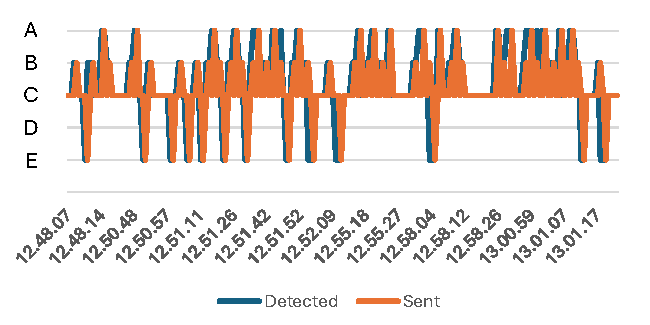
\includegraphics[width=1\textwidth]{gambar/tex/sents.pdf}
    \caption{Detection and Transmission Plots.}
    \label{fig:detection_transmission_plots}
\end{figure}

Visualisasi pada gambar \ref{fig:detection_transmission_plots} berperan penting dalam mendeteksi adanya anomali atau kesalahan yang mungkin terjadi selama proses pengujian. Data yang dipilih untuk divisualisasikan merupakan salah satu hasil terbaik dari serangkaian percobaan terpisah yang telah dilakukan. Hal ini menunjukkan bahwa data tersebut merepresentasikan kondisi sistem yang optimal dan relevan untuk dianalisis lebih lanjut.

\begin{table}[H]
    \centering
    \caption{Summary of Data Transmission and Detection}
    \label{tab:summary_data_transmission_detection}
    \begin{tabular}{|c|c|}
        \hline 
        \cellcolor[HTML]{000000} & \cellcolor[HTML]{C0C0C0} \textbf{Percentage}   \\ \hline
        \cellcolor[HTML]{C0C0C0} \textbf{Transmitted as \texttt{C}} & 55.4  \\ \hline
        \cellcolor[HTML]{C0C0C0} \textbf{Same Register}  & 38.3 \\ \hline
        \cellcolor[HTML]{C0C0C0} \textbf{Different Register}  & 6.3 \\ \hline
    \end{tabular}
\end{table}

Tabel \ref{tab:summary_data_transmission_detection} merangkum data transmisi dan deteksi. Persentase data yang dikirim sebagai \texttt{C} adalah 55.4\%, yang menunjukkan bahwa sistem sering mengirim instruksi untuk berhenti. Persentase data di mana deteksi dan data yang dikirim sama adalah 38.3\%, yang menunjukkan bahwa sistem berjalan sesuai dengan deteksi yang dilakukan. Persentase data di mana deteksi dan data yang dikirim berbeda adalah 6.3\%, yang menunjukkan adanya galat atau kesalahan dalam sistem.

\newpage
\subsection{Percobaan Bergerak Maju}
\label{subsec:percobaanbergerakmaju}

Bagian ini membahas kemampuan sistem dalam mengikuti objek yang bergerak maju dengan kecepatan konstan. Tantangan yang dihadapi adalah bagaimana sistem mempertahankan objek dalam frame sambil melakukan penyesuaian kecepatan yang diperlukan. Solusinya meliputi pemanfaatan fusi data dari YOLOv11 dan MediaPipe Pose, serta penerapan algoritma kontrol yang mampu melakukan koreksi arah tepat waktu, sehingga sistem dapat mengikuti objek yang bergerak maju dengan stabil dan akurat.

\begin{table}[H]
    \centering
    \caption{Data Performa Bergerak Maju}
    \label{tab:performa_bergerak_maju}
    \begin{tabular}{|c|c|c|c|c|c|c|c|}
    \hline
    Waktu & Reg (s) & YOLO (m) & MP (m) & x (px) & Deteksi & Terkirim & Keterangan \\ \hline
    12.48.09 & 0.2991 & 5.6875 & 46.1146 & 484 & b'B\textbackslash n' & b'E\textbackslash n' & Forward \\ \hline
    12.48.10 & 0.2516 & 2.2093 & 5.6063 & 595 & b'B\textbackslash n' & b'C\textbackslash n' & Forward \\ \hline
    12.48.17 & 2.6621 & 1.7109 & 3.1479 & 447 & b'B\textbackslash n' & b'C\textbackslash n' & Forward \\ \hline
    12.50.45 & 0.5046 & 2.5900 & 5.4523 & 391 & b'B\textbackslash n' & b'C\textbackslash n' & Forward \\ \hline
    12.50.46 & 0.3870 & 2.5980 & 4.9960 & 414 & b'B\textbackslash n' & b'B\textbackslash n' & Forward \\ \hline
    12.50.54 & 2.5388 & 1.4768 & 3.1208 & 501 & b'B\textbackslash n' & b'C\textbackslash n' & Forward \\ \hline
    12.51.00 & 0.3556 & 1.7144 & 1.5984 & 492 & b'B\textbackslash n' & b'C\textbackslash n' & Forward \\ \hline
    12.51.00 & 0.3290 & 1.4978 & 1.4964 & 466 & b'B\textbackslash n' & b'B\textbackslash n' & Forward \\ \hline
    12.51.08 & 0.3129 & 1.6801 & 1.7017 & 525 & b'B\textbackslash n' & b'C\textbackslash n' & Forward \\ \hline
    12.51.09 & 0.3226 & 1.6408 & 1.7256 & 463 & b'B\textbackslash n' & b'B\textbackslash n' & Forward \\ \hline
    12.51.17 & 5.5467 & 2.2628 & 2.6525 & 563 & b'B\textbackslash n' & b'C\textbackslash n' & Forward \\ \hline
    12.51.17 & 0.3035 & 1.9853 & 2.1709 & 408 & b'B\textbackslash n' & b'B\textbackslash n' & Forward \\ \hline
    12.51.21 & 2.9916 & 2.0186 & 3.1728 & 440 & b'B\textbackslash n' & b'C\textbackslash n' & Forward \\ \hline
    12.51.21 & 0.3446 & 2.4830 & 3.1701 & 601 & b'B\textbackslash n' & b'B\textbackslash n' & Forward \\ \hline
    12.51.26 & 3.8579 & 2.5354 & 2.0134 & 553 & b'B\textbackslash n' & b'C\textbackslash n' & Forward \\ \hline
    12.51.30 & 3.3993 & 2.4258 & 2.4468 & 551 & b'B\textbackslash n' & b'C\textbackslash n' & Forward \\ \hline
    12.51.36 & 4.6957 & 1.7144 & 1.8941 & 478 & b'B\textbackslash n' & b'C\textbackslash n' & Forward \\ \hline
    12.51.42 & 0.2820 & 1.4820 & 2.5157 & 424 & b'B\textbackslash n' & b'C\textbackslash n' & Forward \\ \hline
    12.51.42 & 0.2867 & 1.5473 & 1.6206 & 481 & b'B\textbackslash n' & b'B\textbackslash n' & Forward \\ \hline
    12.51.44 & 0.2619 & 1.6003 & 1.9633 & 426 & b'B\textbackslash n' & b'A\textbackslash n' & Forward \\ \hline
    12.51.45 & 0.2692 & 1.5704 & 1.6022 & 449 & b'B\textbackslash n' & b'C\textbackslash n' & Forward \\ \hline
    12.51.51 & 2.5508 & 2.2628 & 1.8379 & 569 & b'B\textbackslash n' & b'C\textbackslash n' & Forward \\ \hline
    12.51.52 & 0.6972 & 1.9174 & 2.2452 & 394 & b'B\textbackslash n' & b'B\textbackslash n' & Forward \\ \hline
    12.51.55 & 0.3125 & 1.9262 & 2.1721 & 564 & b'B\textbackslash n' & b'C\textbackslash n' & Forward \\ \hline
    12.52.05 & 0.2830 & 1.9395 & 2.9075 & 502 & b'B\textbackslash n' & b'C\textbackslash n' & Forward \\ \hline
    12.55.13 & 0.3498 & 2.0186 & 1.9290 & 520 & b'B\textbackslash n' & b'C\textbackslash n' & Forward \\ \hline
    12.55.14 & 0.3321 & 1.8664 & 2.8010 & 511 & b'B\textbackslash n' & b'B\textbackslash n' & Forward \\ \hline
    12.55.18 & 0.2536 & 1.2489 & 1.0783 & 483 & b'B\textbackslash n' & b'C\textbackslash n' & Forward \\ \hline
    12.55.18 & 0.3409 & 1.2734 & 1.0403 & 522 & b'B\textbackslash n' & b'B\textbackslash n' & Forward \\ \hline
    12.55.22 & 0.3309 & 1.5194 & 3.5842 & 504 & b'B\textbackslash n' & b'C\textbackslash n' & Forward \\ \hline
    \end{tabular}
\end{table}

Tabel \ref{tab:performa_bergerak_maju} menunjukkan data performa sistem saat bergerak maju. Data ini mencakup waktu deteksi, jarak deteksi dari YOLOv11 dan MediaPipe Pose, posisi objek dalam frame, hasil deteksi, instruksi yang dikirimkan, dan keterangan mengenai arah gerak. Data ini memberikan gambaran kinerja sistem dalam mengikuti objek yang bergerak maju, termasuk kecepatan respons, akurasi deteksi, dan ketepatan instruksi yang dikirimkan.

\begin{figure}[H]
    \centering
    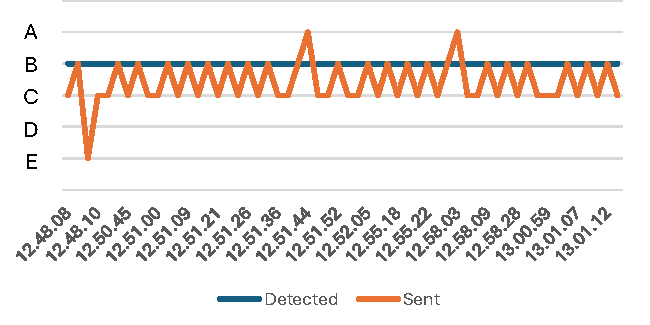
\includegraphics[width=1\textwidth]{gambar/tex/forward.pdf}
    \caption{Straight Movement Plots}
    \label{fig:straight_movement_plots}
\end{figure}

Visualisasi pada gambar \ref{fig:straight_movement_plots} berperan penting dalam mendeteksi adanya anomali atau kesalahan yang mungkin terjadi selama proses pengujian. Data yang dipilih untuk divisualisasikan merupakan salah satu hasil terbaik dari serangkaian percobaan terpisah yang telah dilakukan. Hal ini menunjukkan bahwa data tersebut merepresentasikan kondisi sistem yang optimal dan relevan untuk dianalisis lebih lanjut.

\begin{table}[H]
    \centering
    \caption{Summary of Data During Straight Movement}
    \label{tab:straight_movement_data_transmission_detection}
    \begin{tabular}{|c|c|}
        \hline 
        \cellcolor[HTML]{000000} & \cellcolor[HTML]{C0C0C0} \textbf{Percentage}   \\ \hline
        \cellcolor[HTML]{C0C0C0} \textbf{Transmitted as \texttt{C}} & 15.4  \\ \hline
        \cellcolor[HTML]{C0C0C0} \textbf{Same Register}  & 11.0  \\ \hline
        \cellcolor[HTML]{C0C0C0} \textbf{Different Register}   & 1.5  \\ \hline
    \end{tabular}
\end{table}

Tabel \ref{tab:straight_movement_data_transmission_detection} merangkum data transmisi dan deteksi selama gerakan maju. Persentase data yang dikirim sebagai \texttt{C} adalah 15.4\%, yang menunjukkan bahwa sistem sering mengirim instruksi untuk berhenti. Persentase data di mana deteksi dan data yang dikirim sama adalah 11.0\%, yang menunjukkan bahwa sistem berjalan sesuai dengan deteksi yang dilakukan. Persentase data di mana deteksi dan data yang dikirim berbeda adalah 1.5\%, yang menunjukkan adanya galat atau kesalahan dalam sistem.

\newpage
\subsection{Percobaan Belok Kiri}
\label{subsec:percobaanbelokkiri}

Bagian ini membahas kemampuan sistem dalam mengikuti objek saat berbelok ke kiri. Pada kondisi ini, tantangan yang muncul meliputi perubahan posisi relatif yang terjadi lebih cepat, potensi kehilangan objek dari frame, serta perlunya adaptasi kecepatan motor penggerak. Solusi yang diterapkan adalah penyesuaian parameter kontrol, algoritma pendeteksi pose yang lebih adaptif, serta strategi gerak yang mempertimbangkan arah belok objek sehingga sistem dapat mempertahankan jarak optimal dan ketepatan manuver ke kiri.

\begin{table}[H]
    \centering
    \caption{Data Performa Belok (Kiri)}
    \label{tab:performa_belok_kiri}
    \begin{tabular}{|c|c|c|c|c|c|c|c|c|}
    \hline
    Waktu & Reg (s) & YOLO (m) & MP (m) & x (px) & Deteksi & Terkirim & Keterangan \\ \hline
    12:48:14 & 2.7739 & 1.4513 & 1.1409 & 128 & b'A\textbackslash n' & b'C\textbackslash n' & Turn Left \\ \hline
    12:50:48 & 2.7333 & 1.1421 & 1.0733 & 164 & b'A\textbackslash n' & b'C\textbackslash n' & Turn Left \\ \hline
    12:51:18 & 0.3176 & 1.6668 & 1.1184 & 189 & b'A\textbackslash n' & b'C\textbackslash n' & Turn Left \\ \hline
    12:51:18 & 0.3818 & 1.5277 & 1.1295 & 202 & b'A\textbackslash n' & b'A\textbackslash n' & Turn Left \\ \hline
    12:51:26 & 0.4472 & 1.9174 & 1.4873 & 212 & b'A\textbackslash n' & b'C\textbackslash n' & Turn Left \\ \hline
    12:51:27 & 0.2536 & 1.6668 & 1.2112 & 142 & b'A\textbackslash n' & b'A\textbackslash n' & Turn Left \\ \hline
    12:51:37 & 1.7377 & 1.5194 & 1.4537 & 182 & b'A\textbackslash n' & b'B\textbackslash n' & Turn Left \\ \hline
    12:51:44 & 0.3591 & 2.1528 & 1.7878 & 245 & b'A\textbackslash n' & b'C\textbackslash n' & Turn Left \\ \hline
    12:51:45 & 0.3616 & 1.8259 & 1.5129 & 249 & b'A\textbackslash n' & b'B\textbackslash n' & Turn Left \\ \hline
    12:51:52 & 0.3755 & 1.5912 & 1.3909 & 185 & b'A\textbackslash n' & b'C\textbackslash n' & Turn Left \\ \hline
    12:51:52 & 0.3613 & 1.4716 & 1.2101 & 174 & b'A\textbackslash n' & b'A\textbackslash n' & Turn Left \\ \hline
    12:55:15 & 1.6785 & 1.1238 & 1.0672 & 170 & b'A\textbackslash n' & b'C\textbackslash n' & Turn Left \\ \hline
    12:55:18 & 0.3224 & 1.2129 & 1.4666 & 168 & b'A\textbackslash n' & b'C\textbackslash n' & Turn Left \\ \hline
    12:55:19 & 0.3399 & 1.1515 & 1.3422 & 165 & b'A\textbackslash n' & b'A\textbackslash n' & Turn Left \\ \hline
    12:55:25 & 0.4715 & 1.1164 & 1.4924 & 170 & b'A\textbackslash n' & b'C\textbackslash n' & Turn Left \\ \hline
    12:58:05 & 0.4054 & 1.3446 & 1.3906 & 174 & b'A\textbackslash n' & b'A\textbackslash n' & Turn Left \\ \hline
    12:58:10 & 1.2931 & 1.4123 & 1.6479 & 320 & b'A\textbackslash n' & b'C\textbackslash n' & Turn Left \\ \hline
    12:58:25 & 4.1776 & 1.1047 & 1.2300 & 197 & b'A\textbackslash n' & b'C\textbackslash n' & Turn Left \\ \hline
    12:58:26 & 0.6310 & 1.1284 & 1.2368 & 195 & b'A\textbackslash n' & b'A\textbackslash n' & Turn Left \\ \hline
    13:00:55 & 1.9408 & 1.0975 & 1.0855 & 185 & b'A\textbackslash n' & b'C\textbackslash n' & Turn Left \\ \hline
    13:00:55 & 0.4380 & 1.0975 & 1.1142 & 177 & b'A\textbackslash n' & b'C\textbackslash n' & Turn Left \\ \hline
    13:00:56 & 0.3263 & 1.0960 & 1.1078 & 167 & b'A\textbackslash n' & b'A\textbackslash n' & Turn Left \\ \hline
    13:00:58 & 0.2737 & 1.6903 & 1.0003 & 215 & b'A\textbackslash n' & b'B\textbackslash n' & Turn Left \\ \hline
    13:00:59 & 0.2535 & 1.6869 & 1.4439 & 228 & b'A\textbackslash n' & b'C\textbackslash n' & Turn Left \\ \hline
    13:00:59 & 0.3323 & 1.7536 & 1.3650 & 225 & b'A\textbackslash n' & b'A\textbackslash n' & Turn Left \\ \hline
    13:01:00 & 0.3113 & 1.2734 & 1.1814 & 173 & b'A\textbackslash n' & b'B\textbackslash n' & Turn Left \\ \hline
    13:01:01 & 0.4180 & 1.6188 & 1.0805 & 170 & b'A\textbackslash n' & b'C\textbackslash n' & Turn Left \\ \hline
    13:01:02 & 0.2600 & 1.5882 & 1.5507 & 222 & b'A\textbackslash n' & b'A\textbackslash n' & Turn Left \\ \hline
    13:01:08 & 0.4923 & 1.6188 & 1.3519 & 211 & b'A\textbackslash n' & b'C\textbackslash n' & Turn Left \\ \hline
    13:01:09 & 0.3287 & 1.7039 & 1.7476 & 202 & b'A\textbackslash n' & b'A\textbackslash n' & Turn Left \\ \hline
\end{tabular}
\end{table}

Table \ref{tab:performa_belok_kiri} menunjukkan data performa sistem saat berbelok ke kiri. Data ini mencakup waktu deteksi, jarak deteksi dari YOLOv11 dan MediaPipe Pose, posisi objek dalam frame, hasil deteksi, instruksi yang dikirimkan, dan keterangan mengenai arah belok. Data ini memberikan gambaran kinerja sistem dalam mengikuti objek yang berbelok ke kiri, termasuk kecepatan respons, akurasi deteksi, dan ketepatan instruksi yang dikirimkan.

\begin{figure}[H]
    \centering
    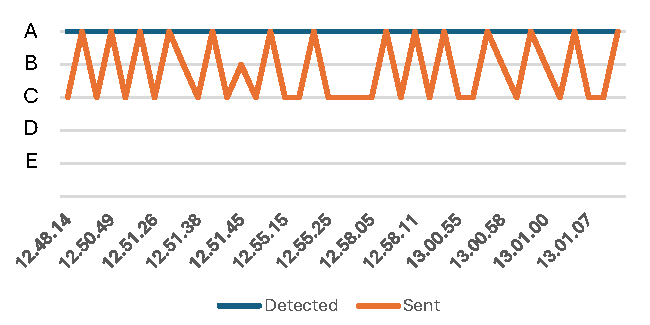
\includegraphics[width=1\textwidth]{gambar/tex/left.pdf}
    \caption{Left Turn Plots}
    \label{fig:left_turn_plots}
\end{figure}

Visualisasi pada gambar \ref{fig:left_turn_plots} berperan penting dalam mendeteksi adanya anomali atau kesalahan yang mungkin terjadi selama proses pengujian. Data yang dipilih untuk divisualisasikan merupakan salah satu hasil terbaik dari serangkaian percobaan terpisah yang telah dilakukan. Hal ini menunjukkan bahwa data tersebut merepresentasikan kondisi sistem yang optimal dan relevan untuk dianalisis lebih lanjut.

\begin{table}[H]
    \centering
    \caption{Summary of Data During Left Turn}
    \label{tab:left_turn_data_transmission_detection}
    \begin{tabular}{|c|c|}
        \hline 
        \cellcolor[HTML]{000000} & \cellcolor[HTML]{C0C0C0} \textbf{Percentage}  \\ \hline
        \cellcolor[HTML]{C0C0C0} \textbf{Transmitted as \texttt{C}} & 10.5 \\ \hline
        \cellcolor[HTML]{C0C0C0} \textbf{Same Register}  & 6.7 \\ \hline
        \cellcolor[HTML]{C0C0C0} \textbf{Different Register}   & 2.0 \\ \hline
    \end{tabular}
\end{table}

Tabel \ref{tab:left_turn_data_transmission_detection} merangkum data transmisi dan deteksi selama belok kiri. Persentase data yang dikirim sebagai \texttt{C} adalah 10.5\%, yang menunjukkan bahwa sistem sering mengirim instruksi untuk berhenti. Persentase data di mana deteksi dan data yang dikirim sama adalah 6.7\%, yang menunjukkan bahwa sistem berjalan sesuai dengan deteksi yang dilakukan. Persentase data di mana deteksi dan data yang dikirim berbeda adalah 2.0\%, yang menunjukkan adanya galat atau kesalahan dalam sistem.

\newpage
\subsection{Percobaan Belok Kanan}
\label{subsec:percobaanbelokkanan}

Bagian ini membahas kemampuan sistem dalam mengikuti objek saat berbelok ke kanan, yang pada dasarnya serupa dengan kondisi belok kanan. Tantangan yang dihadapi adalah bagaimana sistem mempertahankan objek dalam frame sambil melakukan penyesuaian sudut belok yang diperlukan. Solusinya meliputi pemanfaatan fusi data dari YOLOv11 dan MediaPipe Pose, serta penerapan algoritma kontrol yang mampu melakukan koreksi arah tepat waktu, sehingga sistem dapat mengikuti objek yang berbelok ke kanan dengan stabil dan akurat.

\begin{table}[H]
    \centering
    \caption{Data Performa Belok (Kanan)}
    \label{tab:performa_belok_kanan}
    \begin{tabular}{|c|c|c|c|c|c|c|c|c|}
    \hline
    Waktu & Reg (s) & YOLO (m) & MP (m) & x (px) & Deteksi & Terkirim & Keterangan \\ \hline
    12:48:09 & 0.2960 & 2.4469 & 1.6214 & 765 & b'E\textbackslash n' & b'C\textbackslash n' & Turn Right \\ \hline
    12:50:51 & 0.4610 & 1.4219 & 1.0142 & 830 & b'E\textbackslash n' & b'C\textbackslash n' & Turn Right \\ \hline
    12:50:56 & 0.6617 & 2.0234 & 1.6721 & 801 & b'E\textbackslash n' & b'C\textbackslash n' & Turn Right \\ \hline
    12:50:07 & 0.3573 & 1.4291 & 1.4911 & 795 & b'E\textbackslash n' & b'B\textbackslash n' & Turn Right \\ \hline
    12:50:07 & 0.3236 & 1.4588 & 1.7653 & 820 & b'E\textbackslash n' & b'C\textbackslash n' & Turn Right \\ \hline
    12:50:57 & 0.2675 & 2.0939 & 1.4524 & 825 & b'E\textbackslash n' & b'E\textbackslash n' & Turn Right \\ \hline
    12:51:07 & 3.9922 & 1.7796 & 1.3830 & 896 & b'E\textbackslash n' & b'C\textbackslash n' & Turn Right \\ \hline
    12:51:07 & 0.3518 & 2.0345 & 1.5442 & 883 & b'E\textbackslash n' & b'E\textbackslash n' & Turn Right \\ \hline
    12:51:11 & 2.3641 & 1.5332 & 1.5242 & 850 & b'E\textbackslash n' & b'C\textbackslash n' & Turn Right \\ \hline
    12:51:11 & 0.2897 & 2.0453 & 1.7421 & 792 & b'E\textbackslash n' & b'E\textbackslash n' & Turn Right \\ \hline
    12:51:22 & 0.2721 & 2.6141 & 1.7926 & 769 & b'E\textbackslash n' & b'C\textbackslash n' & Turn Right \\ \hline
    12:51:22 & 0.2947 & 2.7330 & 1.5570 & 867 & b'E\textbackslash n' & b'E\textbackslash n' & Turn Right \\ \hline
    12:51:31 & 0.2615 & 2.5602 & 1.3594 & 879 & b'E\textbackslash n' & b'C\textbackslash n' & Turn Right \\ \hline
    12:51:31 & 0.2711 & 2.2042 & 1.3829 & 827 & b'E\textbackslash n' & b'E\textbackslash n' & Turn Right \\ \hline
    12:51:41 & 2.8133 & 1.7721 & 1.4401 & 766 & b'E\textbackslash n' & b'C\textbackslash n' & Turn Right \\ \hline
    12:51:47 & 0.3573 & 1.4291 & 1.4911 & 795 & b'E\textbackslash n' & b'B\textbackslash n' & Turn Right \\ \hline
    12:51:48 & 0.3236 & 1.4588 & 1.7653 & 820 & b'E\textbackslash n' & b'C\textbackslash n' & Turn Right \\ \hline
    12:51:48 & 0.2701 & 1.9485 & 1.6638 & 792 & b'E\textbackslash n' & b'E\textbackslash n' & Turn Right \\ \hline
    12:51:56 & 0.2506 & 1.9262 & 1.7147 & 880 & b'E\textbackslash n' & b'C\textbackslash n' & Turn Right \\ \hline
    12:51:56 & 0.2716 & 1.9759 & 1.6276 & 871 & b'E\textbackslash n' & b'E\textbackslash n' & Turn Right \\ \hline
    12:55:09 & 1.9217 & 1.5004 & 1.8914 & 861 & b'E\textbackslash n' & b'C\textbackslash n' & Turn Right \\ \hline
    12:55:10 & 0.3128 & 2.1414 & 1.8698 & 858 & b'E\textbackslash n' & b'C\textbackslash n' & Turn Right \\ \hline
    12:55:10 & 0.3967 & 2.7356 & 2.0821 & 856 & b'E\textbackslash n' & b'E\textbackslash n' & Turn Right \\ \hline
    12:58:04 & 0.3573 & 1.4291 & 1.4911 & 795 & b'E\textbackslash n' & b'B\textbackslash n' & Turn Right \\ \hline
    12:58:04 & 0.3236 & 1.4588 & 1.7653 & 820 & b'E\textbackslash n' & b'C\textbackslash n' & Turn Right \\ \hline
    12:58:05 & 0.3560 & 1.6768 & 1.8145 & 795 & b'E\textbackslash n' & b'E\textbackslash n' & Turn Right \\ \hline
    13:01:13 & 1.1224 & 1.8459 & 1.5848 & 850 & b'E\textbackslash n' & b'C\textbackslash n' & Turn Right \\ \hline
    13:01:13 & 0.2936 & 1.5942 & 1.0293 & 832 & b'E\textbackslash n' & b'E\textbackslash n' & Turn Right \\ \hline
    13:01:17 & 0.3835 & 1.1238 & 1.0723 & 862 & b'E\textbackslash n' & b'B\textbackslash n' & Turn Right \\ \hline
    13:01:18 & 0.3058 & 1.1253 & 1.0494 & 845 & b'E\textbackslash n' & b'C\textbackslash n' & Turn Right \\ \hline
\end{tabular}
\end{table}

Tabel \ref{tab:performa_belok_kanan} menunjukkan data performa sistem saat berbelok ke kanan. Data ini mencakup waktu deteksi, jarak deteksi dari YOLOv11 dan MediaPipe Pose, posisi objek dalam frame, hasil deteksi, instruksi yang dikirimkan, dan keterangan mengenai arah belok. Data ini memberikan gambaran kinerja sistem dalam mengikuti objek yang berbelok ke kanan, termasuk kecepatan respons, akurasi deteksi, dan ketepatan instruksi yang dikirimkan.

\begin{figure}[H]
    \centering
    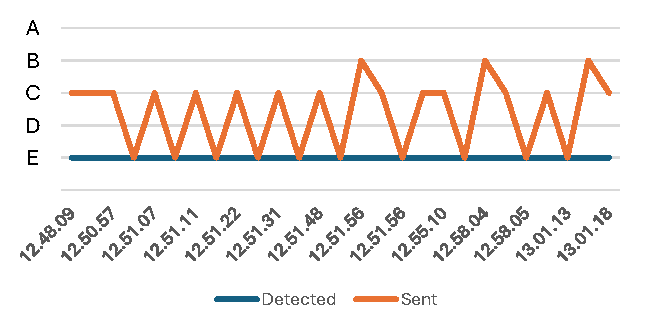
\includegraphics[width=1\textwidth]{gambar/tex/right.pdf}
    \caption{Right Turn Plots}
    \label{fig:right_turn_plots}
\end{figure}

Visualisasi pada gambar \ref{fig:right_turn_plots} berperan penting dalam mendeteksi adanya anomali atau kesalahan yang mungkin terjadi selama proses pengujian. Data yang dipilih untuk divisualisasikan merupakan salah satu hasil terbaik dari serangkaian percobaan terpisah yang telah dilakukan. Hal ini menunjukkan bahwa data tersebut merepresentasikan kondisi sistem yang optimal dan relevan untuk dianalisis lebih lanjut.

\begin{table}[H]
    \centering
    \caption{Summary of Data During Right Turn}
    \label{tab:right_turn_data_transmission_detection}
    \begin{tabular}{|c|c|}
        \hline 
        \cellcolor[HTML]{000000} & \cellcolor[HTML]{C0C0C0} \textbf{Percentage}   \\ \hline
        \cellcolor[HTML]{C0C0C0} \textbf{Transmitted as \texttt{C}} & 6.7  \\ \hline
        \cellcolor[HTML]{C0C0C0} \textbf{Same Register}  & 5.0  \\ \hline
        \cellcolor[HTML]{C0C0C0} \textbf{Different Register}   & 1.5  \\ \hline
    \end{tabular}
\end{table}

Tabel \ref{tab:right_turn_data_transmission_detection} merangkum data transmisi dan deteksi selama belok kanan. Persentase data yang dikirim sebagai \texttt{C} adalah 6.7\%, yang menunjukkan bahwa sistem sering mengirim instruksi untuk berhenti. Persentase data di mana deteksi dan data yang dikirim sama adalah 5.0\%, yang menunjukkan bahwa sistem berjalan sesuai dengan deteksi yang dilakukan. Persentase data di mana deteksi dan data yang dikirim berbeda adalah 1.5\%, yang menunjukkan adanya galat atau kesalahan dalam sistem.

\newpage
\subsection{Percobaan Luar Frame}
\label{subsec:percobaanluarframe}

Bagian ini membahas kemampuan sistem dalam menghadapi kondisi ketika objek keluar dari bidang pandang kamera (luar frame). Tantangan yang muncul adalah hilangnya data visual tentang posisi dan gerakan objek, sehingga sistem harus mampu memprediksi posisi berikutnya atau melakukan penyesuaian strategi pencarian dengan mengintegrasikan algoritma prediksi lintasan serta inisialisasi ulang posisi yang membantu sistem untuk kembali melacak objek setelah objek kembali ke dalam frame.
\begin{table}[H]
    \centering
    \caption{Data Status Frame (Luar Frame)}
    \label{tab:status_luar_frame}
    \begin{tabular}{|c|c|c|c|c|c|c|c|c|}
    \hline
    Waktu & Reg (s) & YOLO (m) & MP (m) & x (px) & Deteksi & Terkirim & Keterangan \\ \hline
    12:48:08 & 0.2758 & 0.0 & 0.0 & 0 & b'B\textbackslash n' & b'B\textbackslash n' & Forward \\ \hline
    12:48:08 & 0.3151 & 0.0 & 0.0 & 0 & b'B\textbackslash n' & b'B\textbackslash n' & Forward \\ \hline
    12:48:15 & 0.2931 & 0.0 & 0.0 & 0 & b'A\textbackslash n' & b'A\textbackslash n' & Turn Left \\ \hline
    12:48:18 & 0.3001 & 0.0 & 0.0 & 0 & b'B\textbackslash n' & b'B\textbackslash n' & Forward \\ \hline
    12:50:43 & 0.7366 & 0.0 & 0.0 & 0 & b'C\textbackslash n' & b'C\textbackslash n' & Stop \\ \hline
    12:50:43 & 0.3732 & 0.0 & 0.0 & 0 & b'C\textbackslash n' & b'C\textbackslash n' & Stop \\ \hline
    12:50:43 & 0.2571 & 0.0 & 0.0 & 0 & b'C\textbackslash n' & b'C\textbackslash n' & Stop \\ \hline
    12:50:44 & 0.2395 & 0.0 & 0.0 & 0 & b'E\textbackslash n' & b'E\textbackslash n' & Turn Right \\ \hline
    12:50:44 & 0.3522 & 0.0 & 0.0 & 0 & b'C\textbackslash n' & b'C\textbackslash n' & Stop \\ \hline
    12:50:44 & 0.3647 & 0.0 & 0.0 & 0 & b'C\textbackslash n' & b'C\textbackslash n' & Stop \\ \hline
    12:50:45 & 0.3504 & 0.0 & 0.0 & 0 & b'C\textbackslash n' & b'C\textbackslash n' & Stop \\ \hline
    12:50:49 & 0.3535 & 0.0 & 0.0 & 0 & b'A\textbackslash n' & b'A\textbackslash n' & Turn Left \\ \hline
    12:51:07 & 0.3518 & 0.0 & 0.0 & 0 & b'E\textbackslash n' & b'E\textbackslash n' & Turn Right \\ \hline
    12:51:11 & 0.2897 & 0.0 & 0.0 & 0 & b'E\textbackslash n' & b'E\textbackslash n' & Turn Right \\ \hline
    12:51:26 & 0.3185 & 0.0 & 0.0 & 0 & b'B\textbackslash n' & b'B\textbackslash n' & Forward \\ \hline
    12:51:30 & 0.2687 & 0.0 & 0.0 & 0 & b'B\textbackslash n' & b'B\textbackslash n' & Forward \\ \hline
    12:51:31 & 0.2615 & 0.0 & 0.0 & 0 & b'E\textbackslash n' & b'E\textbackslash n' & Turn Right \\ \hline
    12:51:31 & 0.2711 & 0.0 & 0.0 & 0 & b'E\textbackslash n' & b'E\textbackslash n' & Turn Right \\ \hline
    12:51:38 & 0.2502 & 0.0 & 0.0 & 0 & b'A\textbackslash n' & b'A\textbackslash n' & Turn Left \\ \hline
    12:51:38 & 0.2617 & 0.0 & 0.0 & 0 & b'A\textbackslash n' & b'A\textbackslash n' & Turn Left \\ \hline
    12:52:05 & 0.6562 & 0.0 & 0.0 & 0 & b'B\textbackslash n' & b'B\textbackslash n' & Forward \\ \hline
    12:58:09 & 0.3319 & 0.0 & 0.0 & 0 & b'B\textbackslash n' & b'B\textbackslash n' & Forward \\ \hline
    12:58:11 & 0.2506 & 0.0 & 0.0 & 0 & b'A\textbackslash n' & b'A\textbackslash n' & Turn Left \\ \hline
    13:00:57 & 0.3574 & 0.0 & 0.0 & 0 & b'C\textbackslash n' & b'C\textbackslash n' & Stop \\ \hline
    13:01:07 & 0.2856 & 0.0 & 0.0 & 0 & b'A\textbackslash n' & b'A\textbackslash n' & Turn Left \\ \hline
    13:01:12 & 0.2639 & 0.0 & 0.0 & 0 & b'B\textbackslash n' & b'B\textbackslash n' & Forward \\ \hline
    13:01:16 & 1.3214 & 0.0 & 0.0 & 0 & b'C\textbackslash n' & b'C\textbackslash n' & Stop \\ \hline
    13:01:16 & 0.3159 & 0.0 & 0.0 & 0 & b'C\textbackslash n' & b'C\textbackslash n' & Stop \\ \hline
    13:01:17 & 0.3360 & 0.0 & 0.0 & 0 & b'C\textbackslash n' & b'C\textbackslash n' & Stop \\ \hline
    13:01:19 & 0.2638 & 0.0 & 0.0 & 0 & b'C\textbackslash n' & b'C\textbackslash n' & Stop \\ \hline
    \end{tabular}
\end{table}
Tabel \ref{tab:status_luar_frame} menunjukkan data status sistem saat objek berada di luar frame. Data ini memperlihatkan saat nilai dari deteksi objek keduanya adalah 0 dan keterangan mengenai status objek. Data ini memberikan gambaran kinerja sistem dalam menghadapi kondisi ketika objek keluar dari bidang pandang kamera.

\section{Performa Keberhasilan Mengikuti}
\label{sec:performamengikuti}

Bagian ini menguji apakah sistem dapat mengikuti objek pada jalur khusus, seperti koridor, area dalam ruangan yang luas, dan jalur landai di sebuah bangunan. Gambar \ref{fig:rute} menunjukkan desain jalur yang disesuaikan untuk akses kursi roda di daerah Tower 2 ITS, mencakup area menuju dan di sekitar lift. Jalur ini memiliki dimensi yang terukur dengan lebar yang cukup untuk manuver kursi roda, termasuk tikungan, ruang untuk berhenti, dan pendekatan ke pintu lift. Jalur dirancang dengan mempertimbangkan radius belok, jarak aman, serta aksesibilitas ke berbagai titik penting seperti lobby dan lift, yang dilengkapi dengan tanda arah yang jelas. Akses ini memastikan kursi roda dapat bergerak dengan nyaman dan aman di seluruh area, termasuk transisi antar ruangan.

\begin{figure}[H]
    \centering
    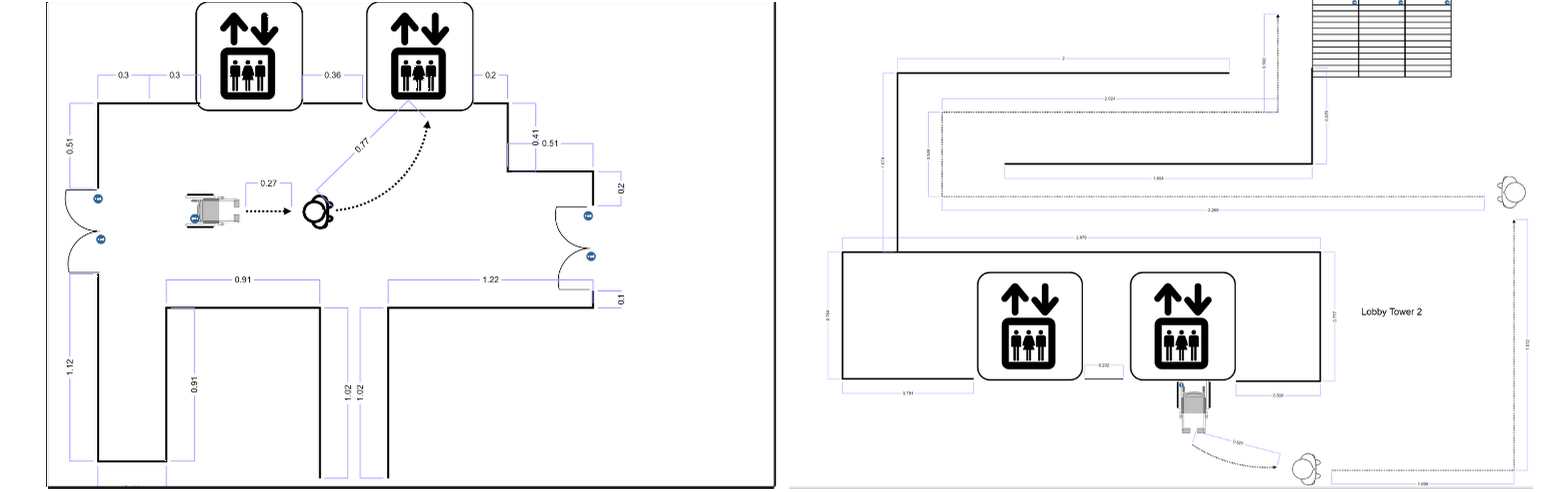
\includegraphics[width=1\textwidth]{gambar/rute.png}
    \caption{Desain Jalur}
    \label{fig:rute}
\end{figure}

Pada gambar \ref{fig:doc_jalur} menunjukkan keberhasilan pengujian kursi roda otonom yang mengikuti pengguna secara real-time. Gambar pertama memperlihatkan kursi roda dengan perangkat elektronik terpasang untuk mendukung fitur otonom, siap untuk diuji. Gambar kedua menunjukkan kursi roda berhasil mengikuti pengguna hingga ke depan lift, menandakan sistem deteksi dan navigasi bekerja dengan baik di lingkungan dalam ruangan. Gambar ketiga mengilustrasikan kursi roda mampu mengikuti pengguna di luar ruangan, termasuk melewati area berbatu dan taman, menunjukkan kemampuan sistem untuk beradaptasi dengan medan yang beragam. Keberhasilan ini mencerminkan integrasi teknologi yang efektif antara perangkat keras dan perangkat lunak.

\begin{figure}[H]
    \centering
    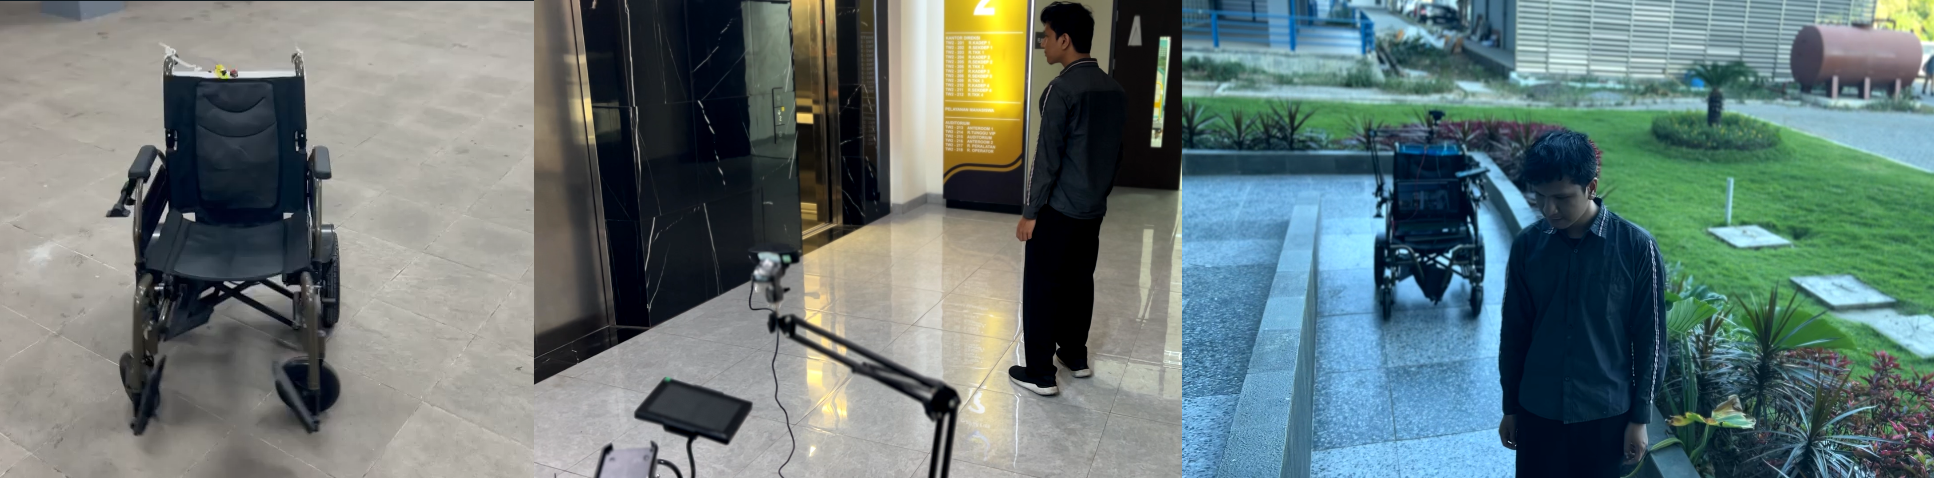
\includegraphics[width=1\textwidth]{gambar/sc_all.png}
    \caption{Dokumentasi Jalur}
    \label{fig:doc_jalur}   
\end{figure}



Pada pengujian ini hasil pengamatan kemudian dirangkum dalam bentuk visual untuk menunjukkan tingkat keberhasilan sistem secara keseluruhan.

\begin{figure}[H]
    \centering
    \begin{tikzpicture}
        \pie[color={green},text=inside, radius=2]{
            100/Sukses
        }
    \end{tikzpicture}
    \caption{Pie Chart Performa Keberhasilan Sistem}
    \label{fig:piechart}
\end{figure}

Hasil pengujian menunjukkan bahwa sistem mampu mengikuti objek dengan baik di seluruh kondisi jalur yang diuji. Visualisasi dalam bentuk pie chart pada Gambar \ref{fig:piechart} mengonfirmasi tingkat keberhasilan sistem mencapai 100\%. Hal ini mencerminkan bahwa sistem memiliki performa yang stabil dan dapat diandalkan untuk beroperasi pada berbagai jenis lingkungan yang telah disimulasikan selama pengujian. Keberhasilan ini menegaskan efektivitas sistem dalam memenuhi tujuan pengembangan untuk mengikuti objek dengan konsisten.

\section{Pembahasan Hasil}
\label{sec:pembahasanhasil}

Pada bagian ini, akan dibahas hasil pengujian yang telah dilakukan terhadap sistem kursi roda otonom berbasis teknik fusi gabungan YOLOv11 dan MediaPipe Pose untuk mendeteksi dan mengikuti manusia. Sistem ini dirancang untuk memanfaatkan kekuatan YOLOv11 dalam mendeteksi objek dengan presisi tinggi serta MediaPipe Pose untuk melacak posisi tubuh manusia secara real-time.

\subsection{Performa Deteksi Objek}
\label{sec:performadeteksiobjek}

Berdasarkan hasil pengujian performa model menggunakan confusion matrix, terlihat bah- wa model YOLOv11 mampu mendeteksi objek manusia dengan tingkat akurasi yang baik. Pada pelatihan dengan 100 epoch, model memiliki box loss sebesar 0.82978 pada tahap training dan 1.199 pada tahap validasi. Skor mAP (mean Average Precision) pada threshold 0.5 mencapai 81.85\%, menunjukkan kemampuan model untuk mendeteksi objek dengan ketepatan yang tinggi.

Visualisasi hasil training dengan confusion matrix menunjukkan bahwa dari 4359 data train dan 1023 data validasi, model berhasil mendeteksi 1806 citra sebagai true positive dan 483 citra sebagai false positive. Pengujian ini mengindikasikan bahwa model cukup efektif dalam mendeteksi manusia, meskipun masih terdapat beberapa kesalahan deteksi.

\subsection{Kecepatan Pemrosesan (FPS)}
\label{sec:kecepatanpemrosesan}

Pengujian kecepatan pemrosesan (FPS) dilakukan pada perangkat laptop sebagai unit komputasi menghasilkan data bahwa sistem mampu memproses frame secara real-time dengan mencatat resolusi frame, jumlah objek yang terdeteksi, dan waktu pemrosesan per frame. Dalam pengujian, sistem mencapai FPS tertinggi sebesar 62,5, dengan rata-rata FPS sekitar 40. Fluktuasi FPS dipengaruhi oleh kondisi lingkungan, kompleksitas objek, dan intensitas perhitungan.

\subsection{Regulator Time}
\label{sec:regulatortime}

Pengujian ini mengukur waktu yang dibutuhkan sistem untuk meregulasi kode isntruksi sesuai dengan perubahan lingkungan, dengan mencatat data arah dan timestamp menggunakan Arduino IDE dan Visual Studio Code. Data yang dihasilkan, berupa Timestamp Receive ESP dan Timestamp Receive Motor, diolah menjadi plot distribusi waktu respons. Hasil pengujian menunjukkan bahwa 66,17\% respons berada dalam waktu yang relatif singkat, sedangkan 34\% lainnya melebihi 0,5 detik, menunjukkan adanya variasi kecil akibat kondisi lingkungan atau performa sistem.

\subsection{Keberhasilan Tracking}
\label{sec:performatracking}

Pengujian ini mengevaluasi keberhasilan sistem dalam melacak target menggunakan BotSORT dan YOLO pada 15 kali percobaan. Sistem berhasil mengunci target (Locked Detection) sebanyak 4 kali, sementara 11 kali terjadi kehilangan fokus (Distracted Detection), menghasilkan tingkat keberhasilan sebesar 26,67\%. Ketidakkonsistenan dalam pelacakan terlihat dari peningkatan nomor track pada setiap objek yang terdeteksi, yang disebabkan oleh kurang optimalnya fungsi \text{track()}. Ketidakmampuan model untuk menjaga identitas ID secara konsisten juga menjadi faktor yang mengurangi akurasi pelacakan secara keseluruhan.

Meskipun demikian, ID yang terdeteksi tetap dapat dimanfaatkan sebagai referensi untuk verifikasi lebih lanjut atau sebagai dasar analisis data. Hal ini memungkinkan sistem untuk tetap memberikan nilai praktis, seperti mendukung identifikasi pola pergerakan atau pengambilan keputusan berbasis data di lingkungan tertentu. Hasil ini menunjukkan bahwa meskipun sistem masih memerlukan peningkatan dalam hal kestabilan pelacakan, termasuk akurasi deteksi, kecepatan respons, dan pengelolaan ID objek, sistem tetap dapat digunakan untuk aplikasi lapangan yang relevan dan memberikan manfaat signifikan.

\subsection{Kesesuaian Tingkat Pencahayaan}
\label{sec:kesesuaianpencahayaan}

Pengujian ini mengevaluasi kemampuan sistem dalam mendeteksi objek pada kondisi pencahayaan yang berbeda, sistem menunjukkan kinerja terbaik pada siang hari ketika tingkat pencahayaan berada pada kondisi optimal, menghasilkan nilai kepercayaan yang lebih tinggi. Sebaliknya, kinerja sistem cenderung menurun pada malam hari akibat kurangnya pencahayaan, yang menyebabkan penurunan nilai kepercayaan pada deteksi objek.

Namun, penggunaan pencahayaan tambahan, seperti senter atau lampu, tidak direkomendasikan karena dapat menyebabkan overexposure pada gambar. Kondisi ini dapat mengurangi akurasi deteksi sistem secara keseluruhan. Oleh karena itu, untuk mencapai performa optimal, penting untuk memastikan bahwa tingkat pencahayaan lingkungan berada dalam rentang yang sesuai tanpa menggunakan pencahayaan buatan yang berlebihan. Hasil pengujian ini menegaskan pentingnya faktor pencahayaan dalam mendukung akurasi sistem deteksi real-time.

\subsection{Kesesuaian Jarak Deteksi}
\label{sec:kesesuaianjarak}

Pengujian menunjukkan bahwa sistem mampu mendeteksi objek dengan jarak kurang dari 1 (satu) meter secara konsisten. Deteksi dilakukan menggunakan YOLOv11 dan MediaPipe Pose, dengan hasil berupa kode instruksi untuk menghentikan sistem ("Stop") guna mencegah tabrakan. Verifikasi tambahan dilakukan dengan pengukuran dan perbandingan dengan alat ukur untuk memastikan akurasi deteksi.

\subsection{Performa Pergerakan Mengikuti Objek}
\label{sec:akurasiikutiobjek}

Evaluasi dilakukan untuk menilai kemampuan sistem dalam mendeteksi objek secara akurat, mengirimkan instruksi yang sesuai, serta menjaga konsistensi kinerja di berbagai kondisi dinamis. Hasil pengujian menunjukkan bahwa:

\begin{itemize}
    \item Pada pengujian dalam frame, sistem mencatat sebagian besar data terkirim sebagai register ‘C’ dengan persentase sebesar 55.4\%, sementara kesalahan transmisi hanya sebesar 6.3\%.
    \item Pada kondisi bergerak maju, instruksi ‘Forward’ terkirim dengan persentase kesalahan transmisi yang sangat kecil, yaitu hanya 1.5\%.
    \item Pada kondisi belok kiri, sistem mencatat data terkirim sebagai register ‘C’ sebesar 10.5\%, dengan kesalahan transmisi sebesar 2.0\%.
    \item Pada kondisi belok kanan, sistem mencatat data terkirim sebagai register ‘C’ sebesar 6.7\%, dengan kesalahan transmisi sebesar 1.5\%.
    \item Saat objek keluar dari frame, sistem mencatat sebagian besar data dengan nilai deteksi nol, dan prioritas diberikan untuk mengirimkan instruksi sebelumnya.
\end{itemize}

Hasil pengujian menunjukkan bahwa sistem memiliki performa yang sangat baik dalam mendeteksi dan mengikuti objek di berbagai skenario, baik saat dalam frame, bergerak maju, maupun berbelok. Sistem mampu menunjukkan stabilitas tinggi dalam transmisi data dan respons yang sesuai terhadap deteksi. Meski demikian, diperlukan perbaikan lebih lanjut dalam menangani kondisi luar frame, terutama untuk mencegah pengiriman instruksi yang tidak relevan atau tidak aman. Dengan pengoptimalan tersebut, sistem akan semakin andal dan aman untuk diterapkan pada berbagai kondisi operasional.

\subsection{Performa Keberhasilan Mengikuti}
\label{sec:keberhasilanmengikuti}

Hasil pengujian menunjukkan bahwa sistem mampu mengikuti objek dengan baik di seluruh kondisi jalur yang diuji, termasuk koridor, area dalam ruangan, dan jalur landai, dengan tingkat keberhasilan mencapai 100\%. Keberhasilan ini menunjukkan efektivitas sistem dalam memenuhi tujuan pengembangan untuk mengikuti objek secara akurat dan stabil, memberikan dasar yang kuat untuk implementasi lebih lanjut pada aplikasi nyata.